\documentclass[a4paper,11pt]{article}
\usepackage{t1enc}
\usepackage[space]{grffile}
\usepackage[round, longnamesfirst]{natbib}  % Bindet den natbib-standard fuer das Zitieren ein
\usepackage{epsfig}
\usepackage{chngcntr}
\usepackage[latin1]{inputenc}   % Ermoeglicht Sonderzeichen direkt einzugeben
\usepackage[T1]{fontenc}        % Garantiert saubere Worttrennung bei Umlauten etc.
\usepackage{color}              % Farbpaket
\usepackage{amsmath,amsfonts,amssymb}   % ermoeglicht mathematische Sonderzeichen
\usepackage[english]{babel}     %
\usepackage{ae}                 %
%\usepackage{graphicx,subfigure}           % Ermoeglicht das Einbinden von Bildern in allen Formaten
\usepackage{graphicx}
\usepackage{longtable}          % zum erstellen von Tabellen ber mehrere Seiten
\usepackage{multirow}           % zum Verbinden von Zeilen innerhalb einer Tabelle
%\usepackage{pictexwd}           % PicTex, ein Graphikpaket
\usepackage{pst-all, multido}   % psTricks, ein Graphikpaket
\usepackage{url}
\usepackage[doublespacing]{setspace}
\usepackage{booktabs,caption,fixltx2e,array,dcolumn}
\usepackage{parskip}
\usepackage{etoolbox}
\usepackage{tabularx}
\usepackage{caption}
\usepackage{subcaption}
%\usepackage{morefloats}
\usepackage[section]{placeins} % Mit FloatBarrier kann verhindert werden, dass Float in der nächsten Section angezeigt werden
\usepackage[bottom]{footmisc} % Fußnoten werden ganz unten angezeigt
\setcitestyle{authoryear, open={((},close={))}}

\newcolumntype{L}[1]{>{\raggedright\arraybackslash}p{#1}} % linksbündig mit Breitenangabe
\newcolumntype{C}[1]{>{\centering\arraybackslash}p{#1}} % zentriert mit Breitenangabe
\newcolumntype{R}[1]{>{\raggedleft\arraybackslash}p{#1}} % rechtsbündig mit Breitenangabe

\makeatletter
\interfootnotelinepenalty 10000
\patchcmd{\Ginclude@eps}{"#1"}{#1}{}{}
\makeatother

\makeatletter
\newcommand\tageq{%
  \ifmeasuring@\else
    \refstepcounter{equation}%
  \fi
  \tag{\theequation}%
}
\makeatother

\newcommand\fnote[1]{\captionsetup{font=tiny}\caption*{#1}}

%\parindent 0cm
%\renewcommand{\baselinestretch}{1}

\renewcommand{\bibnumfmt}[1]{#1.}
\bibpunct{(}{)}{;}{a}{,}{,}

%%%%%%%%%%%%%%%%%%%%%%%%%%%%%%%%%%%%%%%%%%%%%%%%%%%%%%%%%%%%%%%%%%%%%%%%%%%%%%%%%%%%%%%%%%%%%%%%%%%%%%%%%%%%%%%%%%%%%%%%%%%%%%%%%%%%


% ________________ EINRICHTEN DES DOKUMENTS ______________________%

%\bibliographystyle{plainnat}    % legt den Stil fuer das Inhaltsverzeichnis fest

\oddsidemargin 0.0in \evensidemargin 0.0in \textwidth 15.5cm \topmargin -0.8in \textheight 24.5cm
\setlength{\parskip}{1pt}
\setlength{\parindent}{0pt}
\renewcommand{\baselinestretch}{1}


\setlength{\intextsep}{0.5cm} % Legt den Abstand zwischen Gleitobjekten und dem darüber und darunter angeordneten Fließtext fest.

%\oddsidemargin 0.1in \evensidemargin 0.1in \textwidth 15.5cm \topmargin -0.4in \textheight 24.5cm
%\parindent 0cm      % legt die Seitenraender fest

\pagestyle{plain}          % leere Kopfzeile, Seitennummer in der Mitte der Fusszeile

\newcommand{\bs}{\boldsymbol}  % shortcut zur Erzeugung von fetten Sympolen in der Mathe-Umgebung

%\renewcommand{\baselinestretch}{1.25}
% 1,5 -facher Zeilenabstand (Standard ist 1,2-facher Zeilenabstand, also 1,2*1,25 = 1,5

\begin{document}

\pagenumbering{roman}   % roemische Zahlen zur Seitennumerierung


%%%%%%%%%%%%%%%%%%%%%%%%%%%%%%%%%%%%%%%%%%%%%%%%%%%%%%%%%%%%%%%%%%%%%%%%%%%%%%%%%%%%%%%%%%%%%%%%%%%%%%%%%%%%%%%%%%%%%%%%%%%%%%%%%%%%%%%5


\begin{titlepage}       % Umgebung fuer Titelseite, frei gestaltbar

\thispagestyle{empty}   % keine Numerierung auf Titelseite

\begin{center}

\includegraphics[width=13cm]{Bild.png}
\end{center}

\begin{center}

\vspace*{1.5cm}
{\bf  \Large Assignment \#3: Graphical Analysis of Characteristic Functions} \\
\vspace*{2cm} 
\textbf{B473 Numerical Methods in Finance}
\\
Prof. Dr.-Ing. Rainer Sch\"obel
\\
\vspace*{0.5cm} 
Winter Term 2016-2017\\
\end{center}

\vfill
\begin{flushright}
    \emph{Konstantin Smirnov}\\
    \textit{Student-ID: 3980253}\\
     \textit{ Economics and Finance}\\
 T\"ubingen, \today
  




\end{flushright}



% 
% \begin{center}
% $ $			% oeffnet und schliesst eine Matheumgebung (Trick, um den Titel nach unten zu rutschen
% \vspace{4cm}
% 
% {\LARGE TITEL}
% \vskip 4cm
% 
% Diese Seite ist frei gestaltbar
% \end{center}

\end{titlepage}

\newpage                % erzwingt an dieser Stelle einen Seitenumbruch

\listoffigures
\newpage


\tableofcontents

\newpage
\pagenumbering{arabic}      % Seitenzahlen wieder arabisch numerieren
\setcounter{page}{1}        % Ruecksetzen des Seitenzahlzaehlers auf 1
\section{Introduction}
This assignment discusses the idea and application of complex function analysis in order get more insights how Fourier transformation can be applied.

Complex numbers in general can be basically described as a combination of two real numbers (cartesian form):
\begin{equation}
z=x+i*y
\label{cart}
\end{equation}
where are x $\in$ $\mathbb{R}$ and \textit{iy} $\in$ $\mathbb{C}$.
Another representation of complex numbers with respect to (\ref{cart}) is the polar form which is defined as:
\begin{equation}
z=r(\sin \theta + \cos \theta)
\label{polar}
\end{equation}
where r is the radius of the certain point z and $\theta$ is the angle described in radians. Besides this, there are additionally other important representations of complex numbers which will be discussed in this assignment.

The focus of this assignment lays on the discussion of complex functions and its graphical illustrations. Graphical illustrations might face a mapping issue which makes plotting of the functions non-trivial. In the following chapters we will discuss some characteristics of complex functions and its graphical representations.
\section{Complex Exponential Function}
The complex function $\mathsf{e}^z$ is a good introduction of complex analysis. As a starting point of the derivation we use the Taylor-Series expression of the real exponential function (Sch\"obel, 2017):
\begin{equation}
e^{x}=1 + x + \dfrac{x^2}{2!}+\dfrac{x^3}{3!}+\dfrac{x^4}{4!}+...
\label{realTR}
\end{equation}
Applying (\ref{realTR}) on the imaginary part \textit{iy} $\in$ $\mathbb{C}$.
\begin{equation}
e^{iy}=(1 - \dfrac{y^2}{2!}+\dfrac{y^4}{4!}+\dfrac{y^6}{6!})+ i(y - \dfrac{y^3}{3!} + \dfrac{y^5}{5!} - \dfrac{y^7}{3!}
\label{compTR}
\end{equation}
With respect to Taylor-Series expressions of the trigonometric functions sine and cosine, equation (\ref{compTR}) leads to the \textit{Euler Formula}:
\begin{equation}
e^{iy}= \cos y + i \sin y
\label{euler}
\end{equation}
Taking (\ref{realTR}) and (\ref{euler}) together we get a general representation of the complex exponential function:
\begin{equation}
e^{z}=e^{x+iy}=e^{x} (\cos y + i \sin y)
\label{gce}
\end{equation}
Additional, by applying the Euler formula (\ref{euler}) to the polar representation of the complex number (\ref{polar}) one can derive the exponential representation of a complex number:
\begin{equation}
z=re^{i\phi}
\label{gce}
\end{equation}
\subsection{Discussion of Results}
Figures (\ref{plot12}) and (\ref{plot34}) show the complex exponential function in two different representations. All illustrations basically state our derivation of the complex function from above. 

To illustrate the complex function in a 3D space,  we now use $w(z)=e^z$.
Figure \ref{plot12} illustartes the real and complex values of \textit{w(z)} as a representation of the real Re(w) and imaginary part Im(w), respectively. The left figure shows the real space $\mathbb{R}$ values. As you can see, the function follows a cosine function since one peak can be found at 0 on the imaginary y-axis Im(z). This is in line with the theory since the real values of the function are defined in (\ref{gce}) as the cosine of y. On the other hand, you can see in the right plot of figure \ref{plot12} that imaginary part of the function follows a sine function since a peak can be found at $\dfrac{1}{2}\pi$.
\begin{figure}[!h]
\begin{subfigure}[c]{0.5\textwidth}
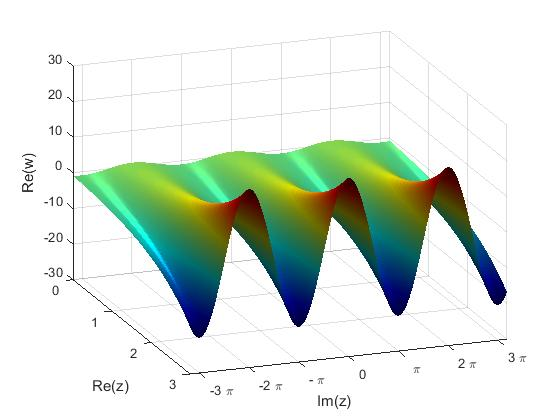
\includegraphics[width=8.5cm]{plot1.jpg}
\subcaption*{Real Part}
\end{subfigure}
\begin{subfigure}[c]{0.5\textwidth}
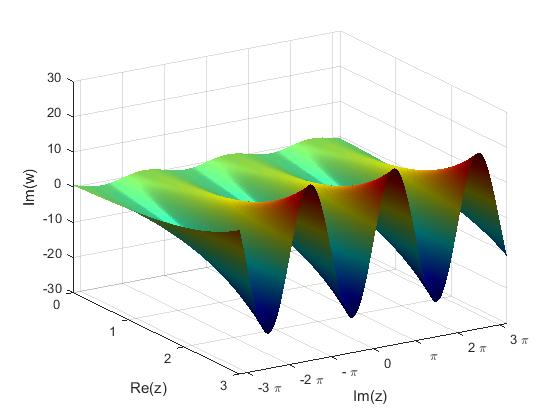
\includegraphics[width=8.5cm]{plot2.jpg}
\subcaption*{Imaginary}
\end{subfigure}
\caption{Complex Exponential Function- Real Part and Imaginary Part}
\label{plot12}
\end{figure}

\begin{figure}[!h]
\begin{subfigure}[c]{0.5\textwidth}
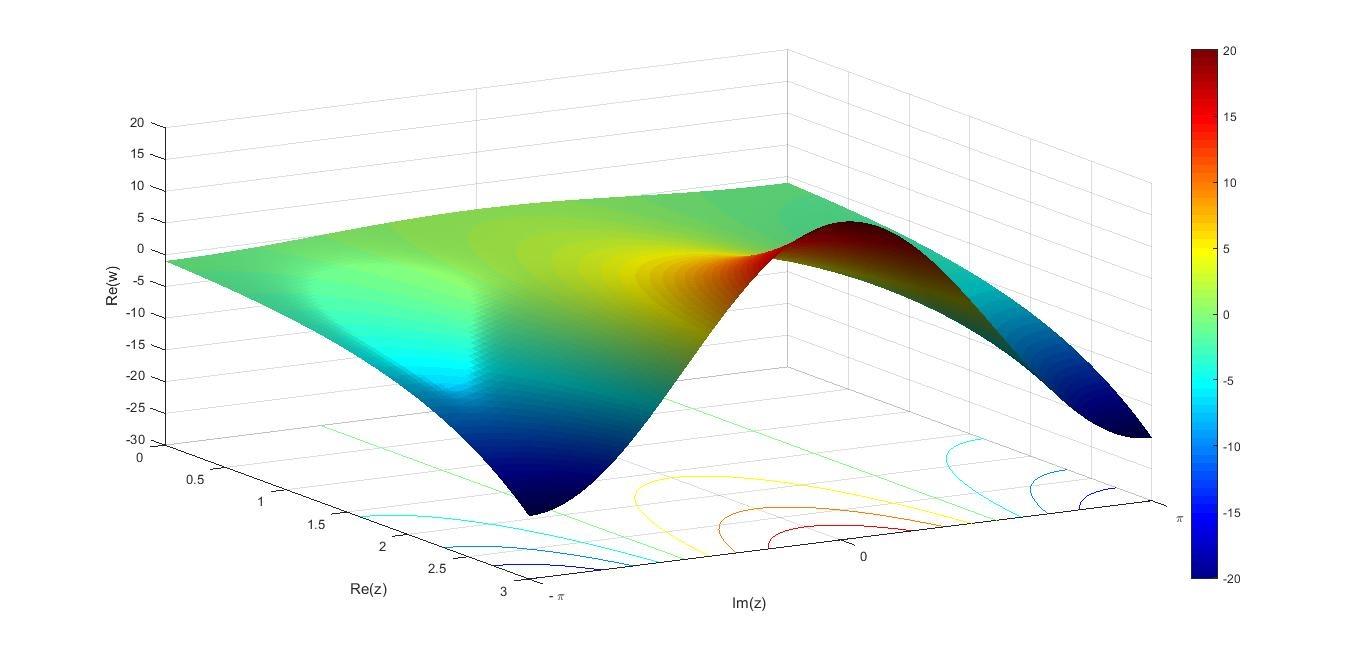
\includegraphics[width=8.5cm]{plot511.jpg}
\subcaption*{Real Part}
\end{subfigure}
\begin{subfigure}[c]{0.5\textwidth}
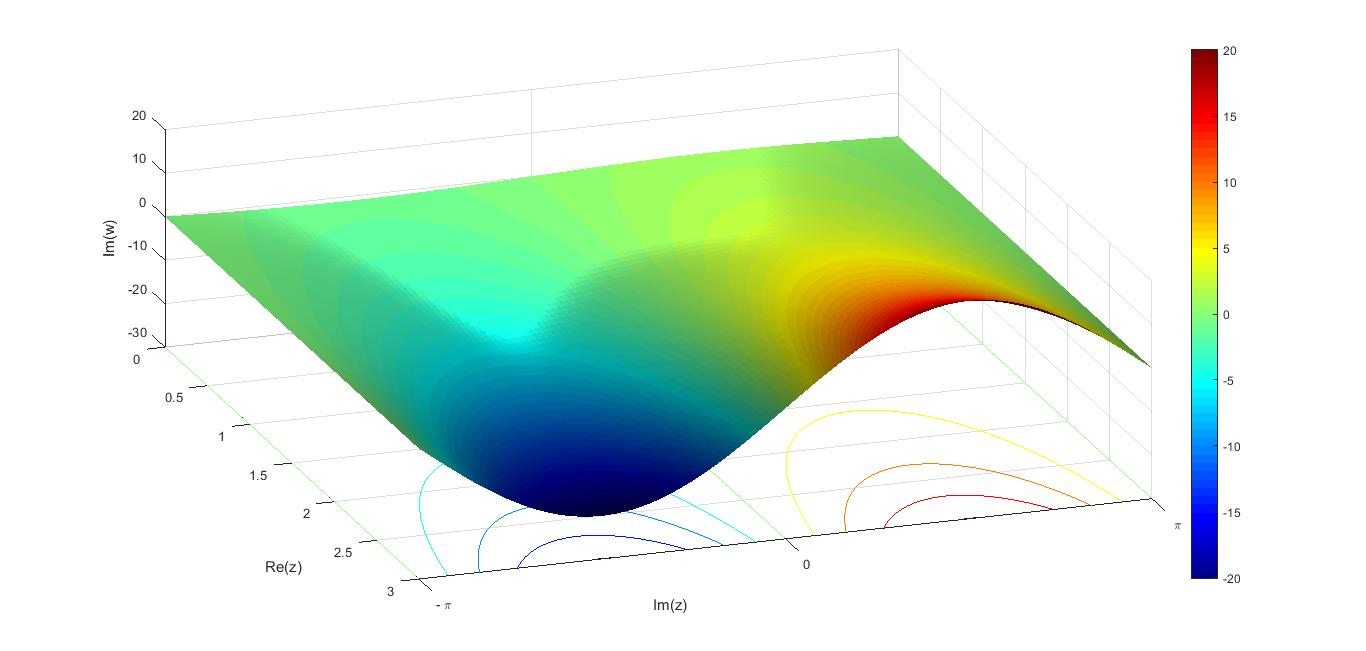
\includegraphics[width=8.5cm]{plot6c.jpg}
\subcaption*{Imaginary}
\end{subfigure}
\caption{Complex Exponential Function- Real Part and Imaginary Part with contours}
\label{plot34}
\end{figure}
Figure \ref{plot34} additionally adds contours to the plots, which support the finding from above. Note that y-axis was restricted to [$-\pi$ $\pi$]  to improve  visualization.  The contours measure the height of the area to precise its behavior. The red contour plot shows that it peaks at $\pi$ and hence represent a cosine function while in the right plot the contour illustrate that it peaks at $\dfrac{1}{2}\pi$, and hence follows a sine function.
\begin{figure}[!h]
\begin{center}
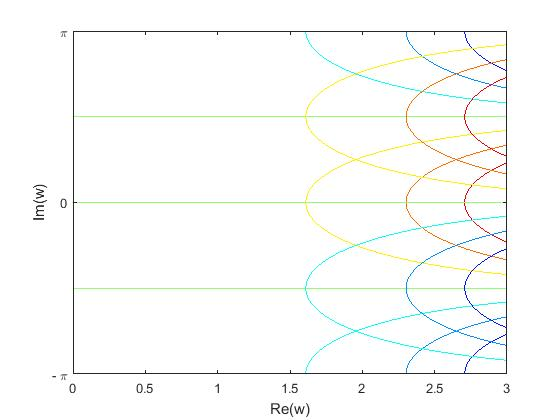
\includegraphics[width=8.5cm]{plot4.jpg}
\caption{Conformal map of $e^z$}
\end{center}
\label{econf}
\end{figure}

Figure 3 combines the contour lines of the left and right illustrations of figure 2 which is another way of illustrating the exponential function. On a range from $-\pi$ to $\pi$ you again see the functional path of cosine and sine. This is a graphical illustration of the Euler formula (\ref{euler}) which was derived in the beginning.
 
\begin{figure}[!h]
\begin{center}
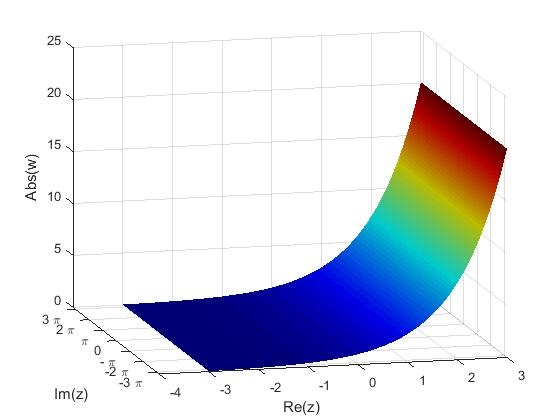
\includegraphics[width=8.5cm]{plot3.jpg}
\caption{Modulus of $e^z$}
\label{plot3}
\end{center}
\end{figure}
Figure \ref{plot3} shows the modulus of $e^z$. As you can clearly see, the illustration follows the same path as the real exponential function. The reason for this is derived as follows. Since the modulus of z can be defined as:
\begin{equation}
|z|=\sqrt{x^2 + y^2}
\label{zmod}
\end{equation}
With respect to the general complex exponential function (\ref{gce}), (\ref{zmod}) leads to
\begin{equation}
|e^{z}|=e^{x}\underbrace{\sqrt{\cos y^2+\sin y^2}}_1=e^x
\end{equation}
Hence the modulus of a complex exponential function is just the real part of the function itself.
\subsection{Technical Implementation}
In this assignment the main script \textit{$Assignment3\_MAIN.m$} was created, where all corresponding function of the assignment are called.

In the first subsection of the main script the function \textit{cexp.m} can be called in order to generate all plots of the first problem. To generate the grid of the function we simply used the \textit{meshgrid} command. It should be mentioned that it was avoided to contain the value 0. Instead the \textit{eps} value was used, which is is a number really close to 0.

In order to plot the graphs we used the \textit{surf, surfc} and and \textit{contour} commands. To distinguish between real, complex and absolute values we simply used the \textit{real, imag or abs} commands, respectively.
\section{Characteristic Function of the Normal Distribution}
In this section we analyse graphically the properties of the characteristic function of the normal distribution.  The characteristic function is the Fourier-transformed Gaussian probability function, which is defined as (Sch\"obel, 2017):
\begin{equation}
w=f(\phi)=exp(-\dfrac{1}{2}\phi^2\sigma^2+i\theta\mu)
\end{equation}
\subsection{Discussion of Results}
In order to compare the behavior of the characteristic function, we varied following parameters:
$\mu$= 0; 1; 4; 16 and $\sigma$=0; 1; 2 on the functional path of $phi$=[0 5].

Illustration \ref{zplane2} show the \textit{z}-values for different parameters of the mean $\mu$ and variance $\sigma^2$ while illustration \ref{wplane2} represents the same combinations but for the functional values \textit{w} .

In the simple cases for $\mu$=0 and $\sigma$=0 we observe in both illustrations a vertical line. This comes simply from the fact that the values at these points are equal to 1 since $e^0$=1 and hence deliver the same values as the functional path.

Speaking generally, following behavior  in figure \ref{zplane2} can be observed:
\begin{itemize}
\item \textit{for increasing $\mu$}: length of the functional path increases and there is more movement on the imaginary part.
\item \textit{for increasing $\sigma^2$}: length and skewness increase due to the parabolic feature of $\sigma^2$ and the direction-angle of the path changes counter-clockwise.
\end{itemize}
\
For the illustrations in figure \ref{wplane2}, we observe following behavior: 
\begin{itemize}
\item \textit{for increasing $\mu$}: the amplitude of the function increases significantly in the imaginary plane since $\mu$ affects the imaginary part of the function. We hence observe more circulation.
\item \textit{for increasing $\sigma^2$}: it affects the movement on the x-axis and circulation decreases.
\end{itemize}
\
\\
Figure \ref{embed2} illustrates how the functional path of the Gaussian distribution fits the exponential function. In this graph the functional path of the characteristic function was embedded to the plots of problem 1. These illustrations show that the Fourier-transformed Gaussian distribution function is just a modified complex exponential function .
\newpage
\begin{figure}[!h]
\begin{subfigure}[c]{0.3\textwidth}
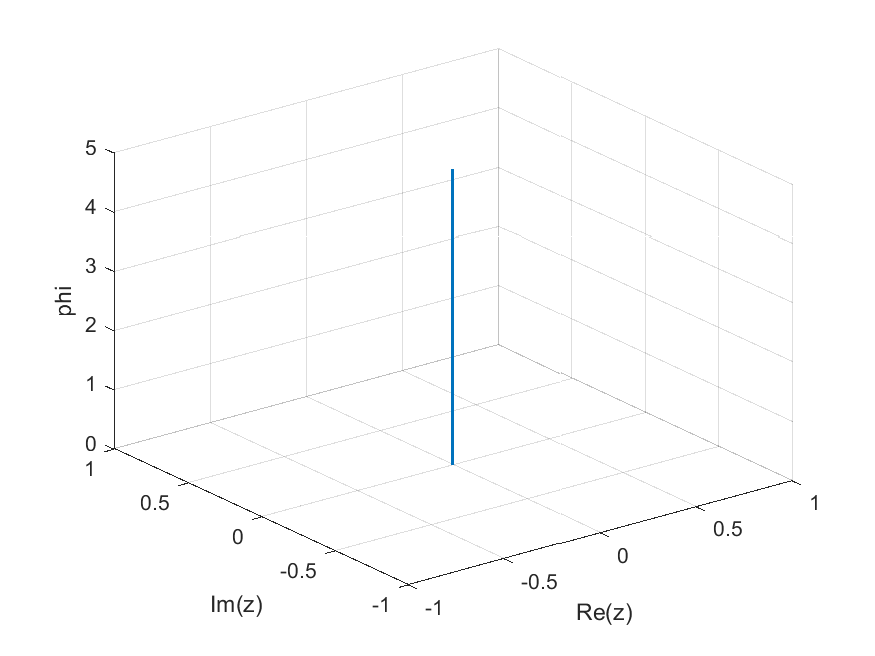
\includegraphics[width=\linewidth]{plot6_musg10.png}
\subcaption*{$\mu$=0 $\sigma$=0 }
\end{subfigure}
\begin{subfigure}[c]{0.3\textwidth}
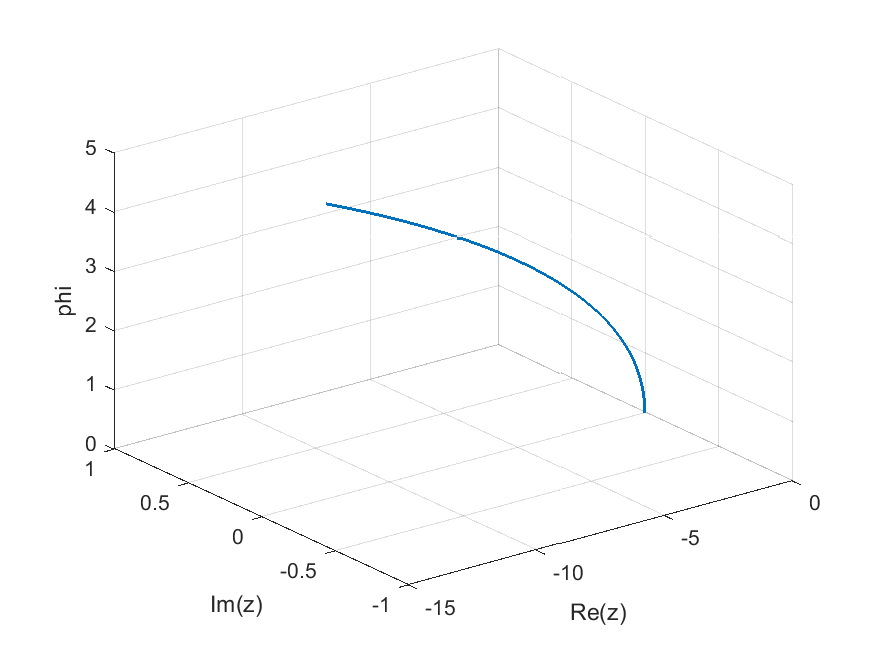
\includegraphics[width=\linewidth]{plot6_musg11.png}
\subcaption*{$\mu$=0 $\sigma$=1 }
\end{subfigure}
\begin{subfigure}[c]{0.3\textwidth}
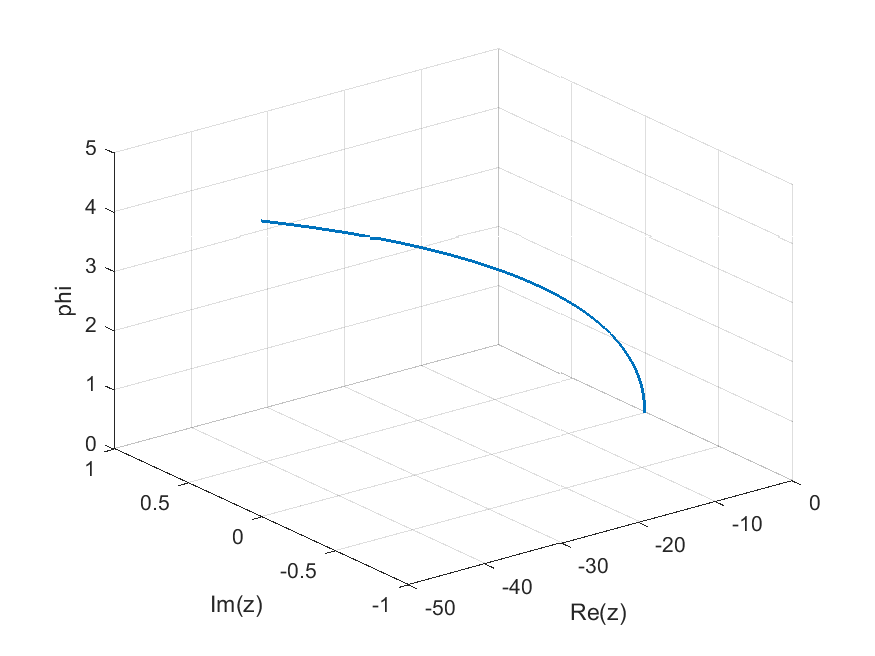
\includegraphics[width=\linewidth]{plot6_musg12.png}
\subcaption*{$\mu$=0 $\sigma$=2 }
\end{subfigure}
\begin{subfigure}[c]{0.3\textwidth}
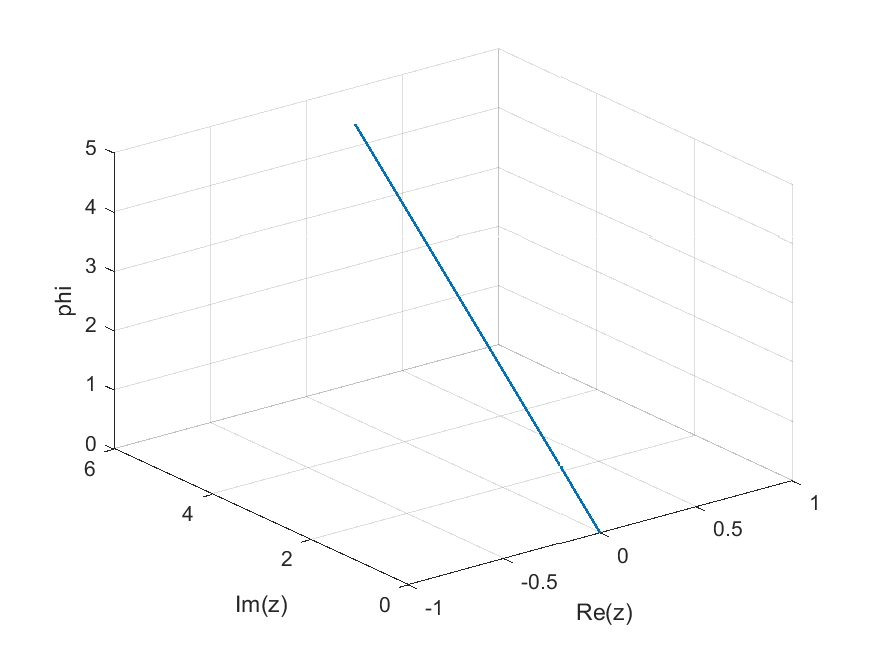
\includegraphics[width=\linewidth]{plot6_musg20.png}
\subcaption*{$\mu$=1 $\sigma$=0 }
\end{subfigure}
\begin{subfigure}[c]{0.3\textwidth}
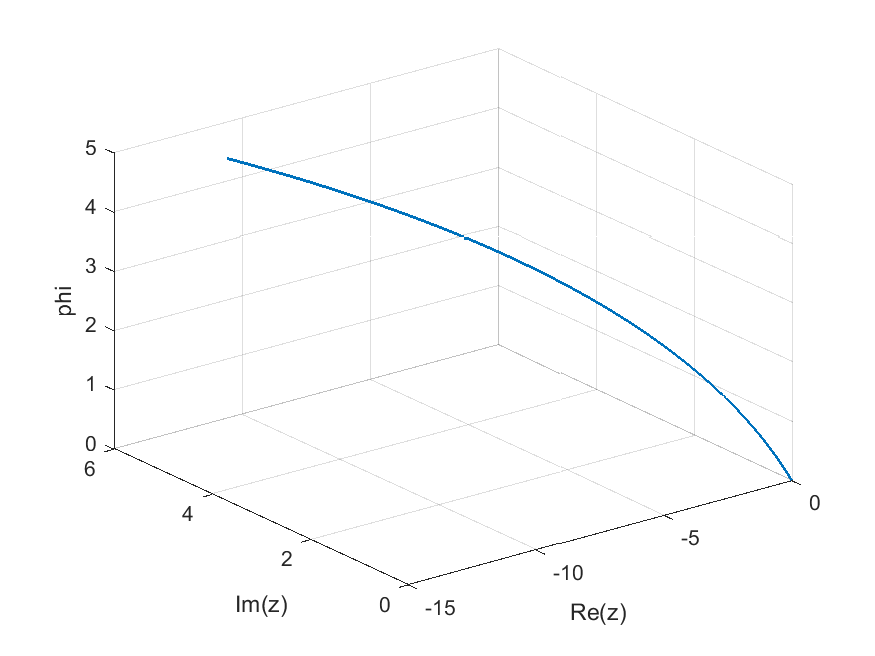
\includegraphics[width=\linewidth]{plot6_musg21.png}
\subcaption*{$\mu$=1 $\sigma$=1 }
\end{subfigure}
\begin{subfigure}[c]{0.3\textwidth}
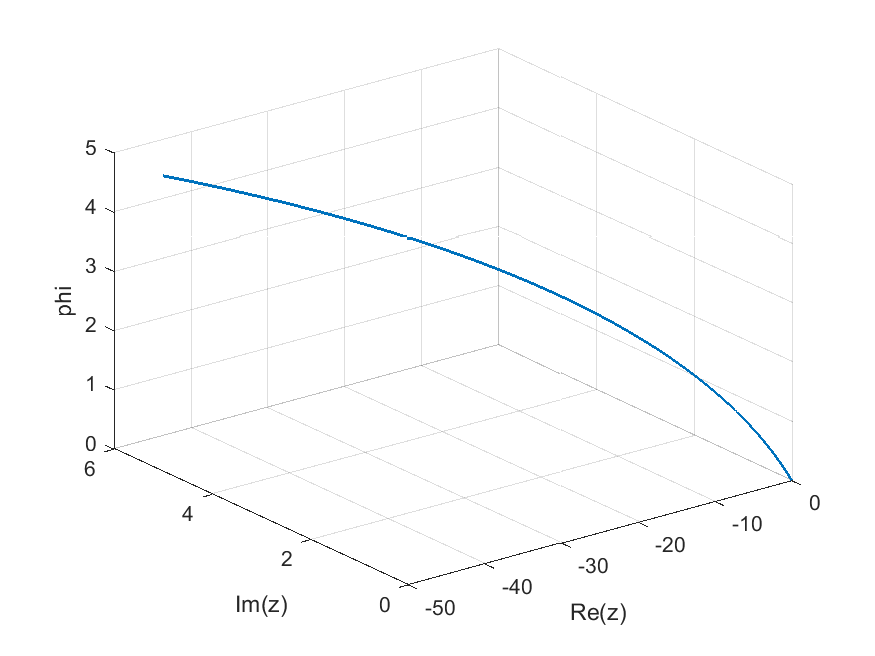
\includegraphics[width=\linewidth]{plot6_musg22.png}
\subcaption*{$\mu$=1 $\sigma$=2 }
\end{subfigure}
\begin{subfigure}[c]{0.3\textwidth}
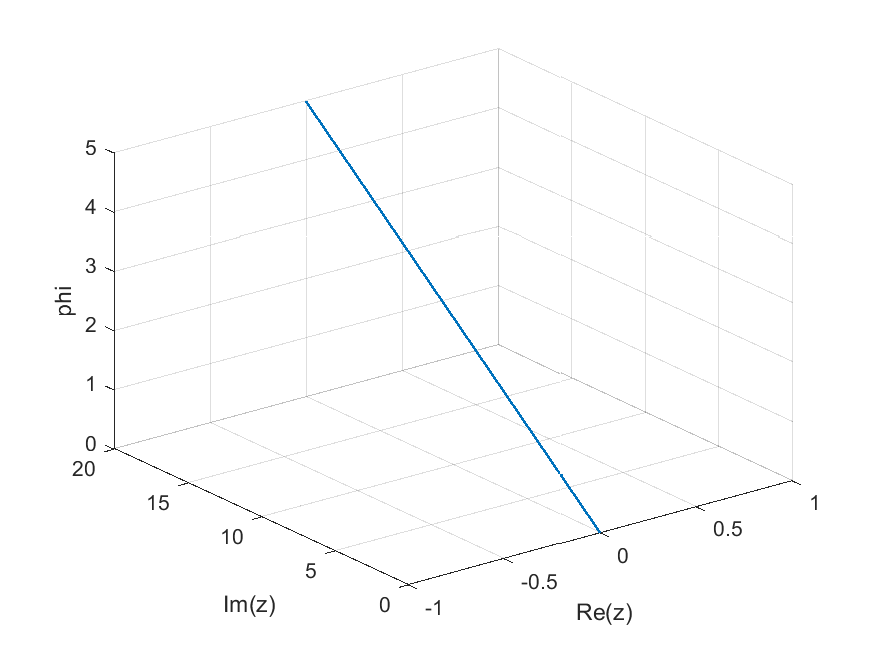
\includegraphics[width=\linewidth]{plot6_musg30.png}
\subcaption*{$\mu$=4 $\sigma$=0 }
\end{subfigure}
\begin{subfigure}[c]{0.3\textwidth}
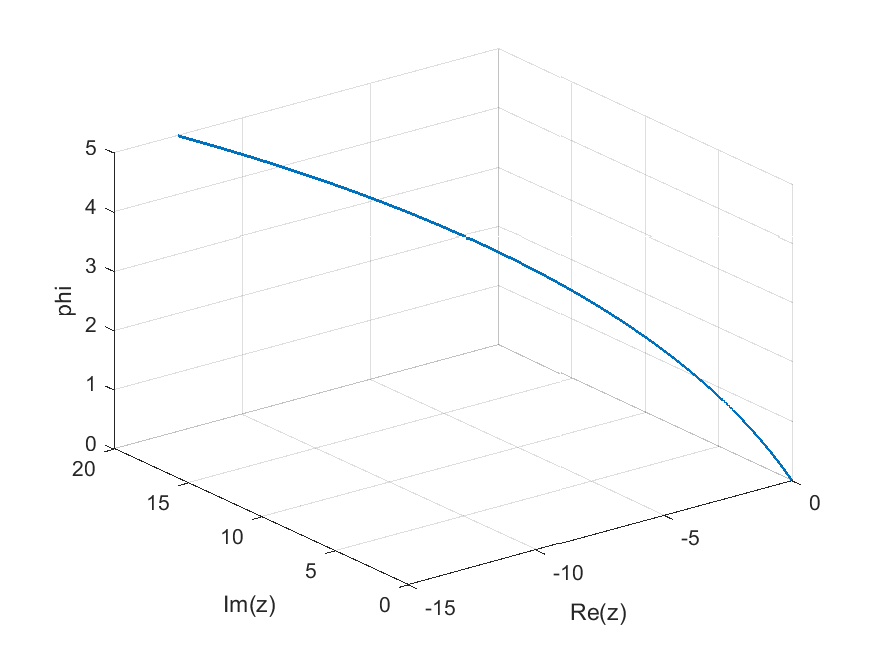
\includegraphics[width=\linewidth]{plot6_musg31.png}
\subcaption*{$\mu$=4 $\sigma$=1 }
\end{subfigure}
\begin{subfigure}[c]{0.3\textwidth}
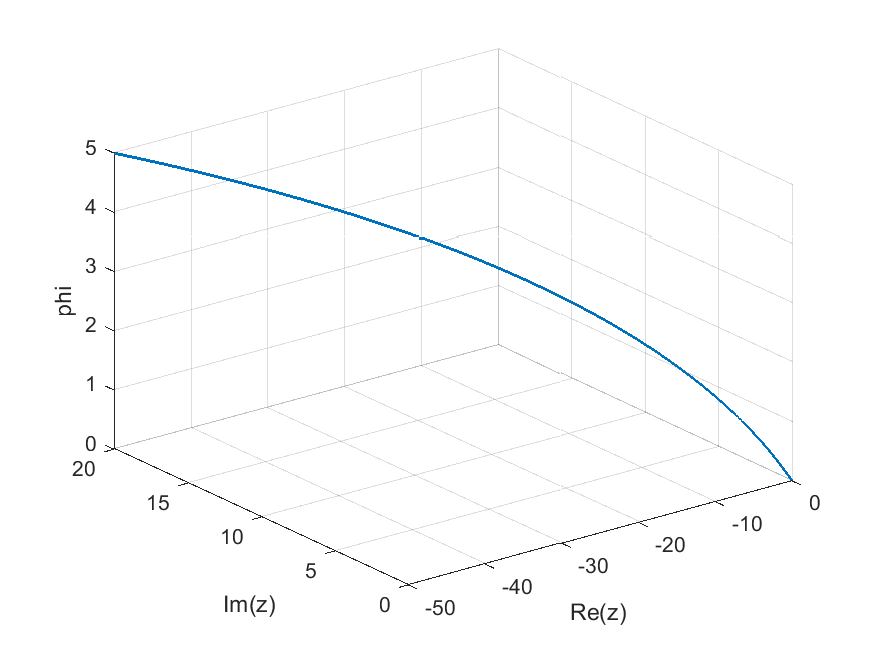
\includegraphics[width=\linewidth]{plot6_musg32.png}
\subcaption*{$\mu$=4 $\sigma$=2 }
\end{subfigure}
\begin{subfigure}[c]{0.3\textwidth}
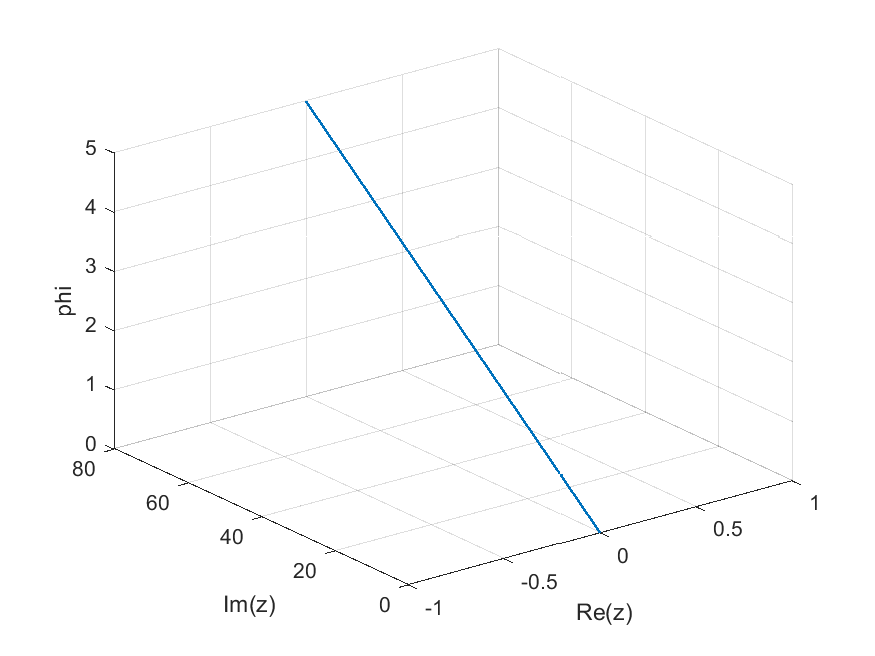
\includegraphics[width=\linewidth]{plot6_musg40.png}
\subcaption*{$\mu$=16 $\sigma$=0 }
\end{subfigure}
\begin{subfigure}[c]{0.3\textwidth}
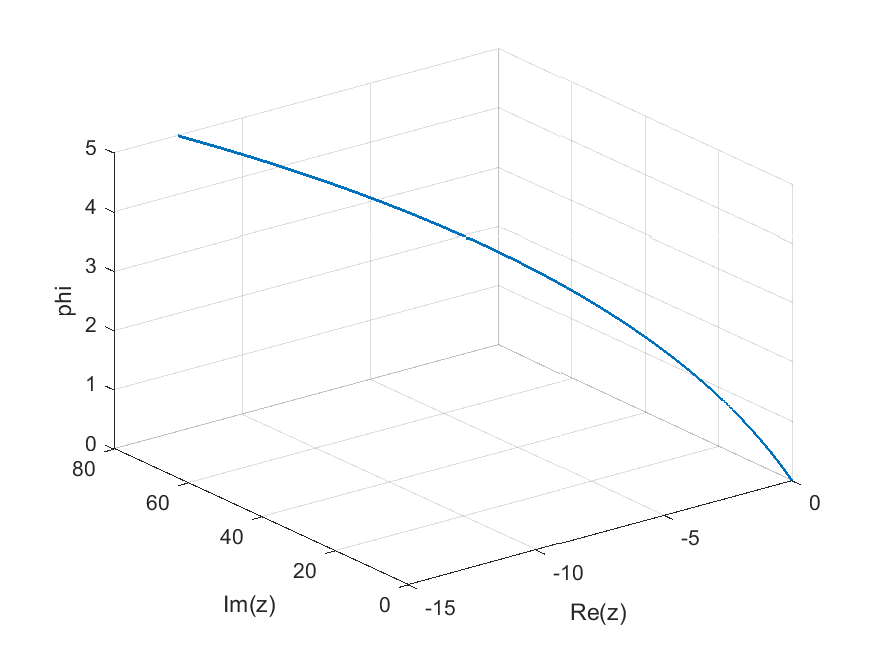
\includegraphics[width=\linewidth]{plot6_musg41.png}
\subcaption*{$\mu$=16 $\sigma$=1 }
\end{subfigure}
\begin{subfigure}[c]{0.3\textwidth}
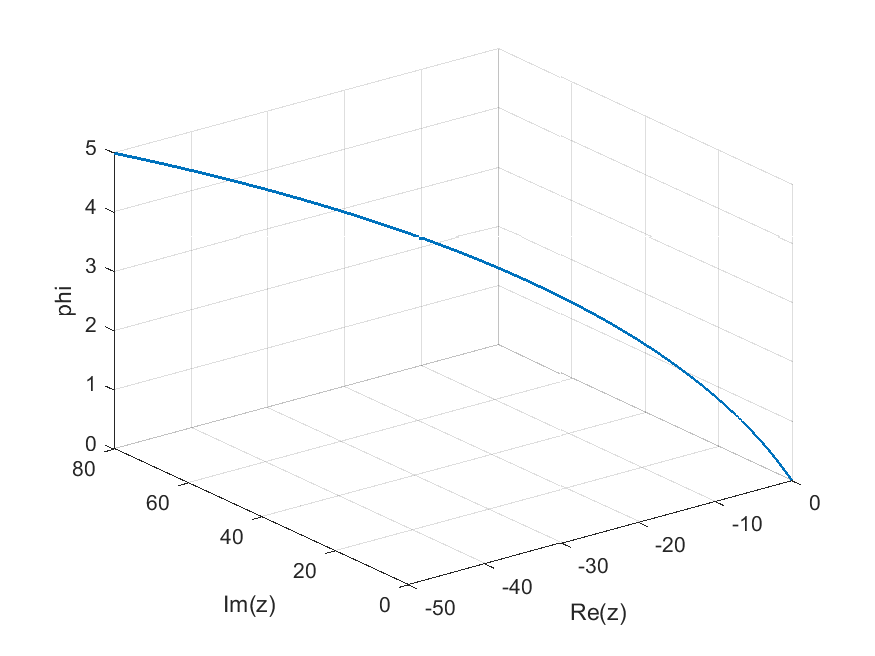
\includegraphics[width=\linewidth]{plot6_musg42.png}
\subcaption*{$\mu$=16 $\sigma$=2 }
\end{subfigure}
\caption{Illustration of the Characteristic Function of the Gaussian Distribution in the z plane}
\label{zplane2}
\end{figure}
\newpage
\newpage
\begin{figure}[!h]
\begin{subfigure}[c]{0.3\textwidth}
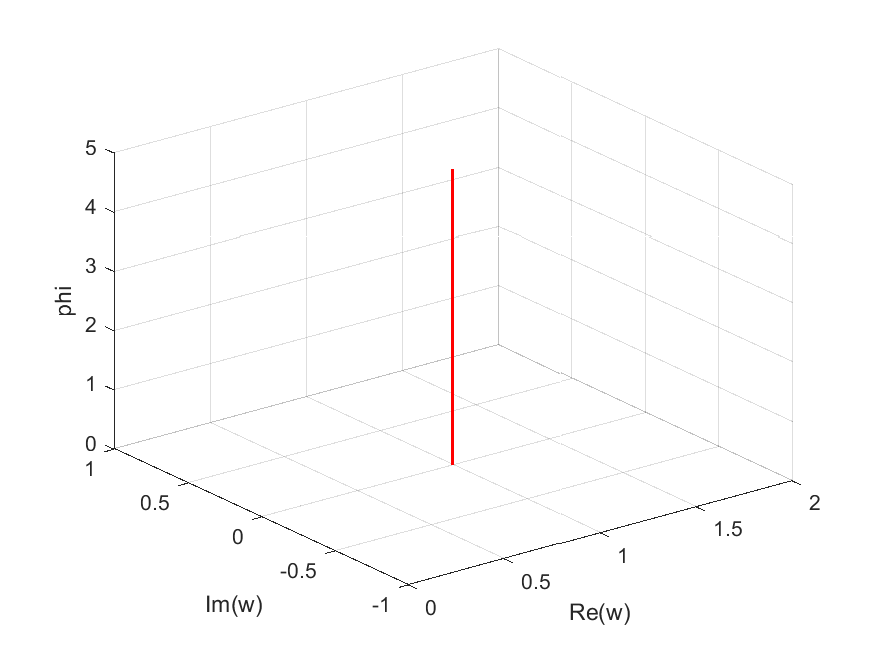
\includegraphics[width=\linewidth]{plot7_musg10.png}
\subcaption*{$\mu$=0 $\sigma$=0 }
\end{subfigure}
\begin{subfigure}[c]{0.3\textwidth}
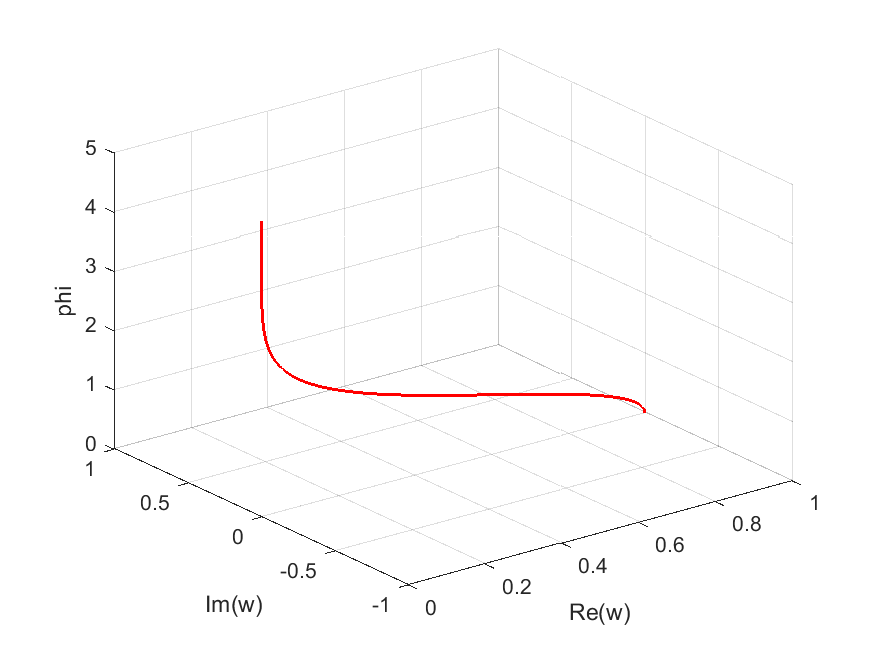
\includegraphics[width=\linewidth]{plot7_musg11.png}
\subcaption*{$\mu$=0 $\sigma$=1 }
\end{subfigure}
\begin{subfigure}[c]{0.3\textwidth}
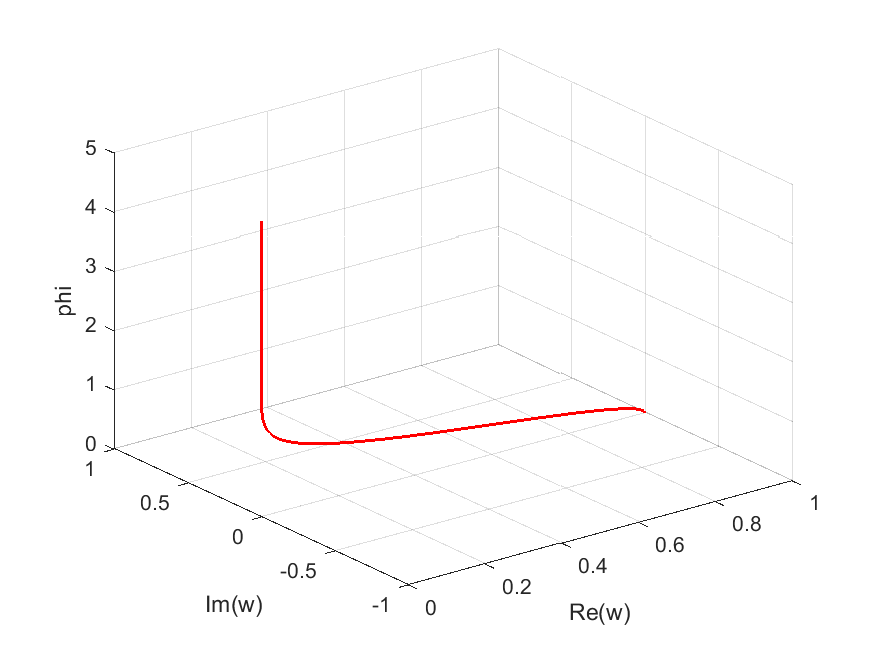
\includegraphics[width=\linewidth]{plot7_musg12.png}
\subcaption*{$\mu$=0 $\sigma$=2 }
\end{subfigure}
\begin{subfigure}[c]{0.3\textwidth}
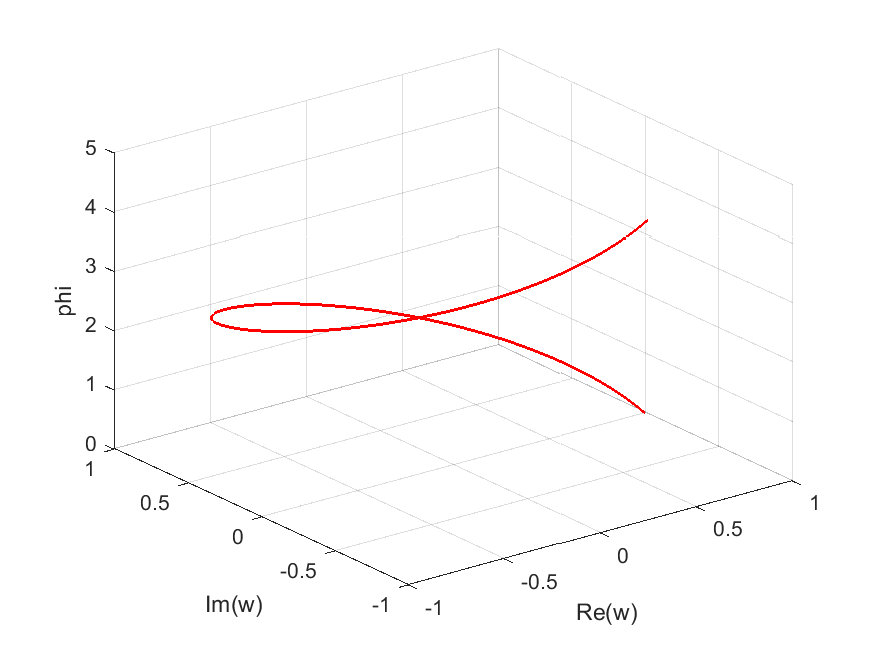
\includegraphics[width=\linewidth]{plot7_musg20.png}
\subcaption*{$\mu$=1 $\sigma$=0 }
\end{subfigure}
\begin{subfigure}[c]{0.3\textwidth}
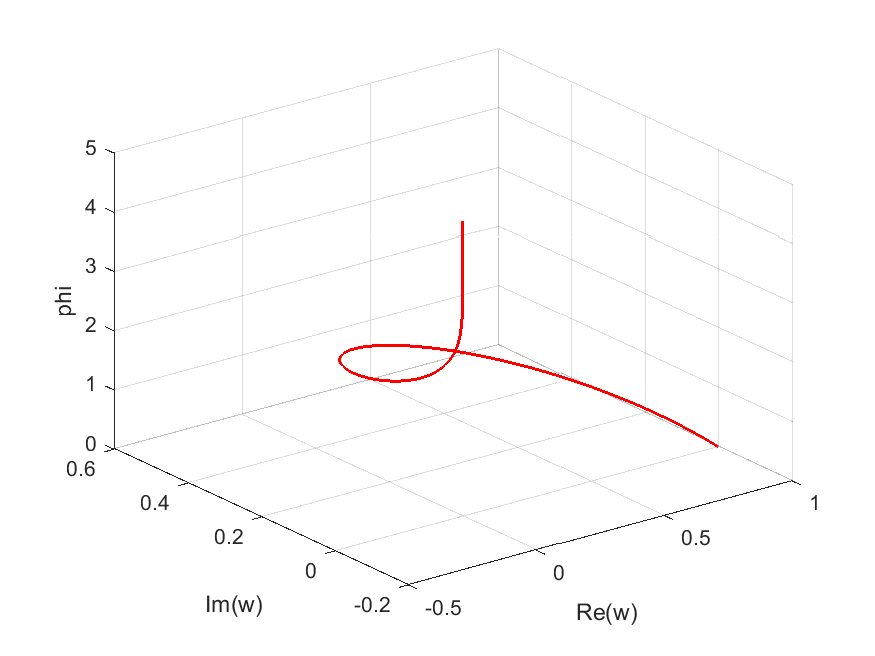
\includegraphics[width=\linewidth]{plot7_musg21.png}
\subcaption*{$\mu$=1 $\sigma$=1 }
\end{subfigure}
\begin{subfigure}[c]{0.3\textwidth}
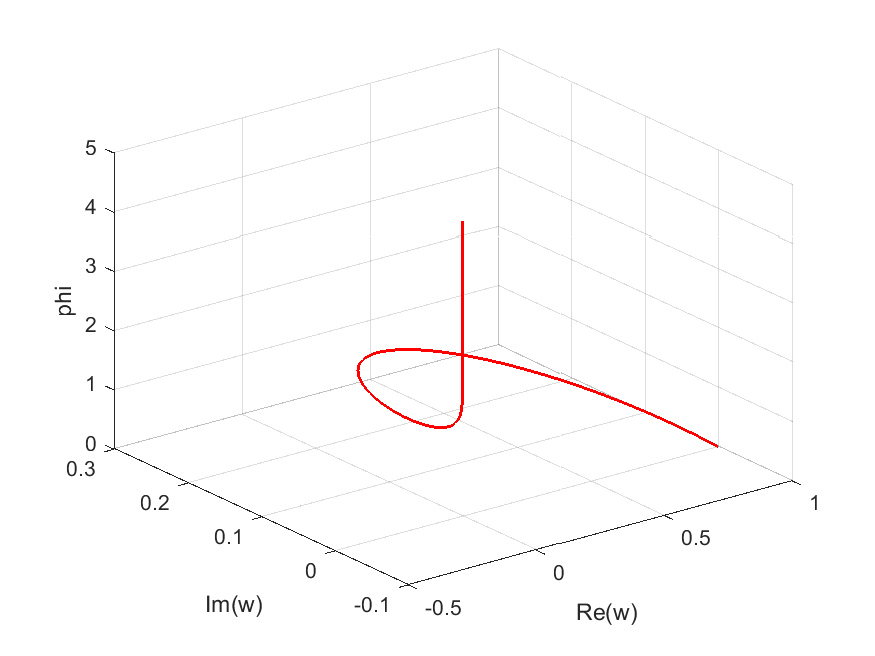
\includegraphics[width=\linewidth]{plot7_musg22.png}
\subcaption*{$\mu$=1 $\sigma$=2 }
\end{subfigure}
\begin{subfigure}[c]{0.3\textwidth}
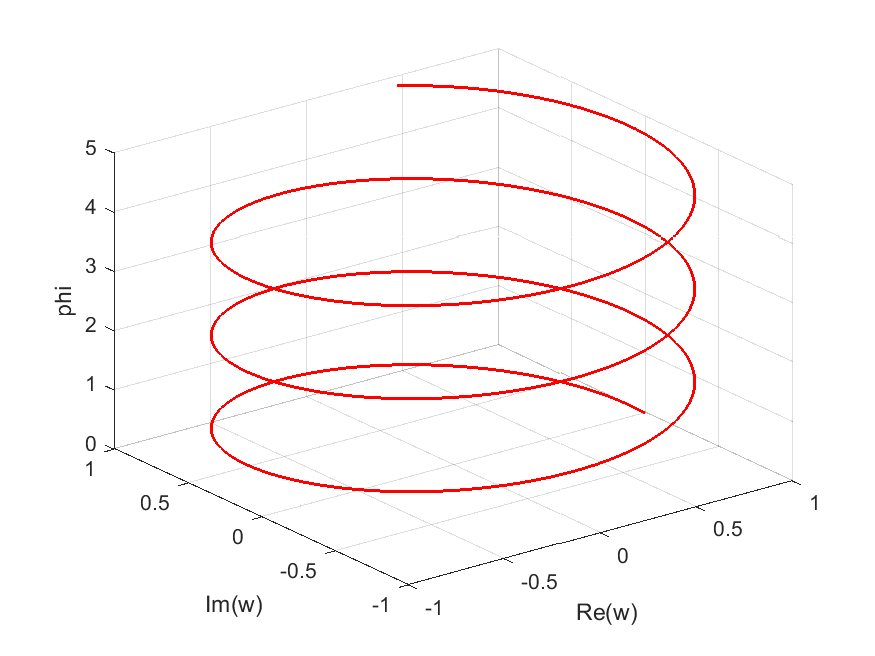
\includegraphics[width=\linewidth]{plot7_musg30.png}
\subcaption*{$\mu$=4 $\sigma$=0 }
\end{subfigure}
\begin{subfigure}[c]{0.3\textwidth}
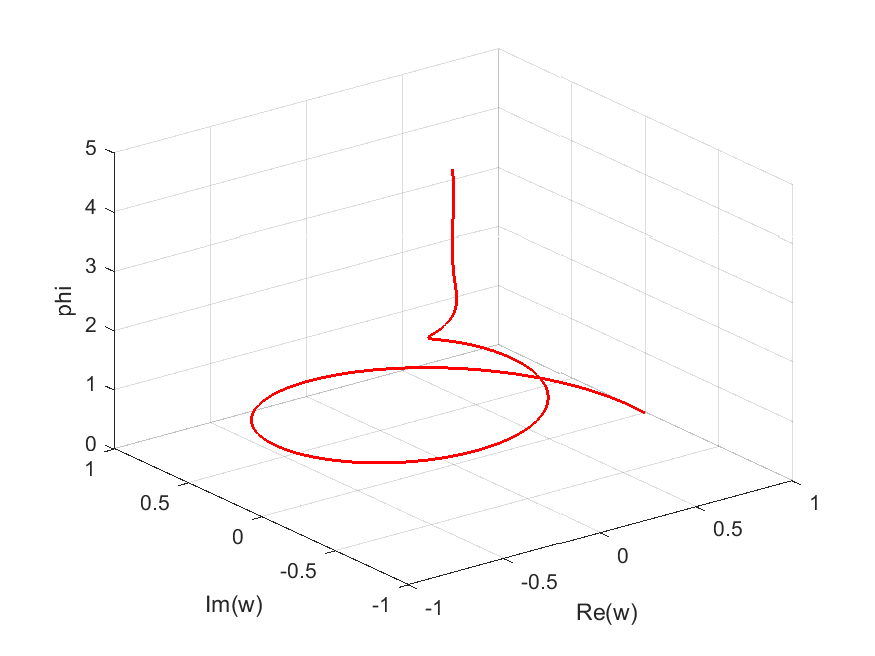
\includegraphics[width=\linewidth]{plot7_musg31.png}
\subcaption*{$\mu$=4 $\sigma$=1 }
\end{subfigure}
\begin{subfigure}[c]{0.3\textwidth}
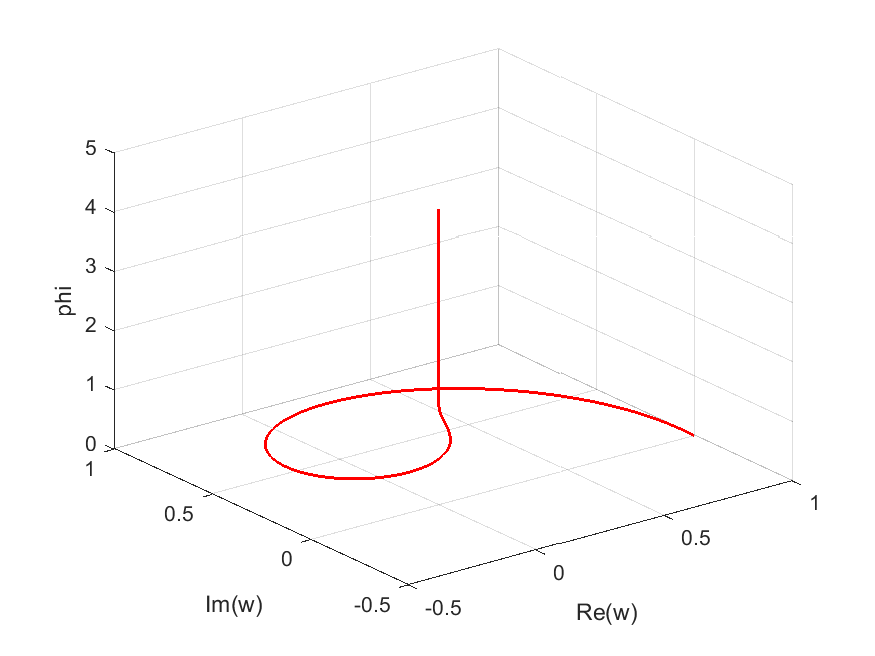
\includegraphics[width=\linewidth]{plot7_musg32.png}
\subcaption*{$\mu$=4 $\sigma$=2 }
\end{subfigure}
\begin{subfigure}[c]{0.3\textwidth}
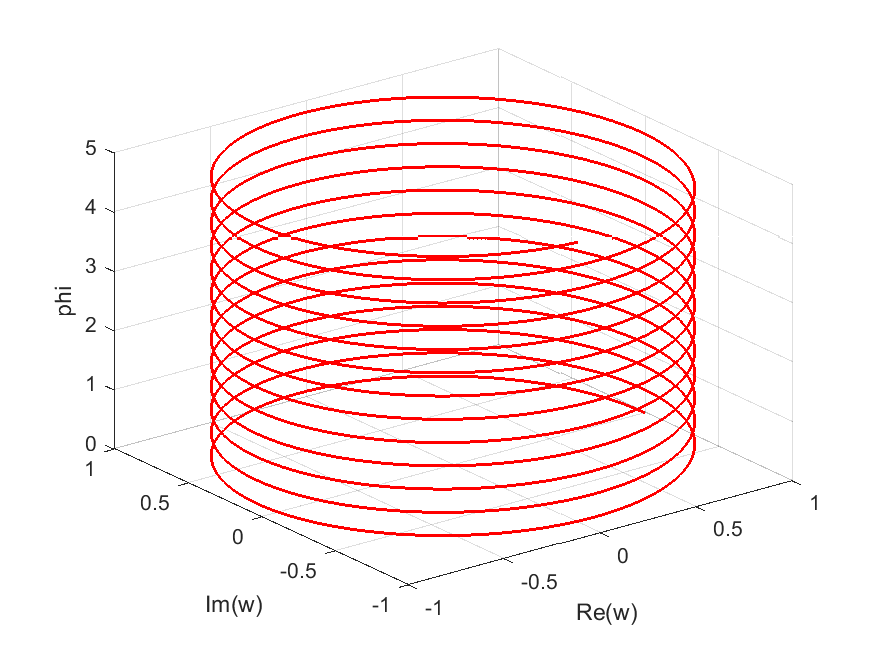
\includegraphics[width=\linewidth]{plot7_musg40.png}
\subcaption*{$\mu$=16 $\sigma$=0 }
\end{subfigure}
\begin{subfigure}[c]{0.3\textwidth}
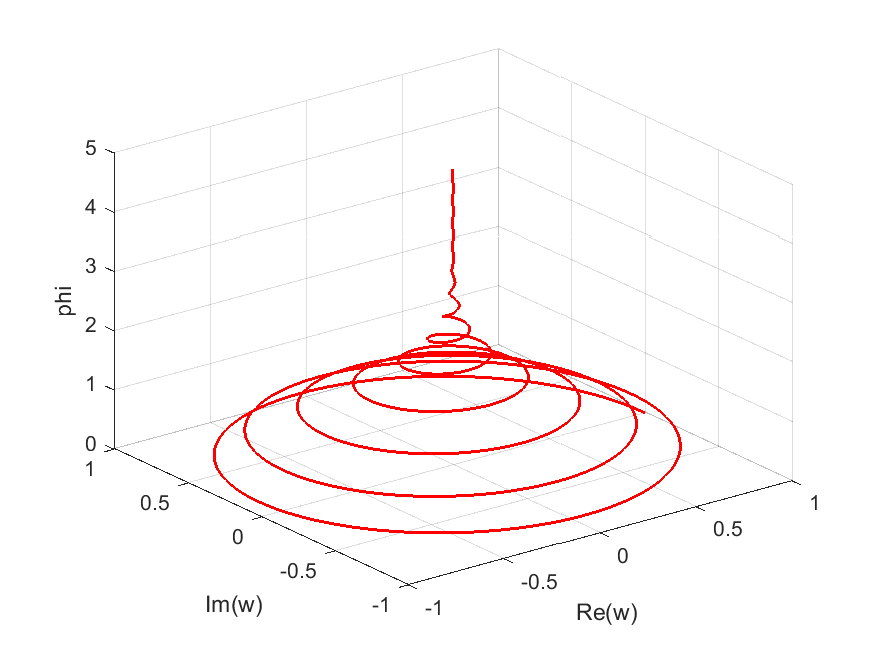
\includegraphics[width=\linewidth]{plot7_musg41.png}
\subcaption*{$\mu$=16 $\sigma$=1 }
\end{subfigure}
\begin{subfigure}[c]{0.3\textwidth}
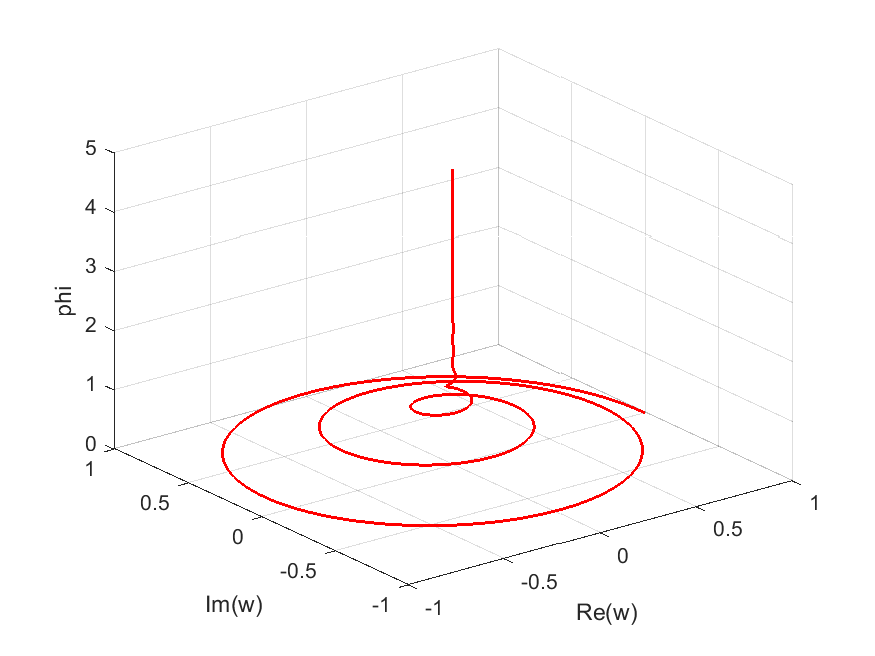
\includegraphics[width=\linewidth]{plot7_musg42.png}
\subcaption*{$\mu$=16 $\sigma$=2 }
\end{subfigure}
\caption{Illustration of the Characteristic Function of the Gaussian Distribution in the w plane}
\label{wplane2}
\end{figure}
\newpage

\begin{figure}[!h]
\begin{subfigure}[c]{0.5\textwidth}
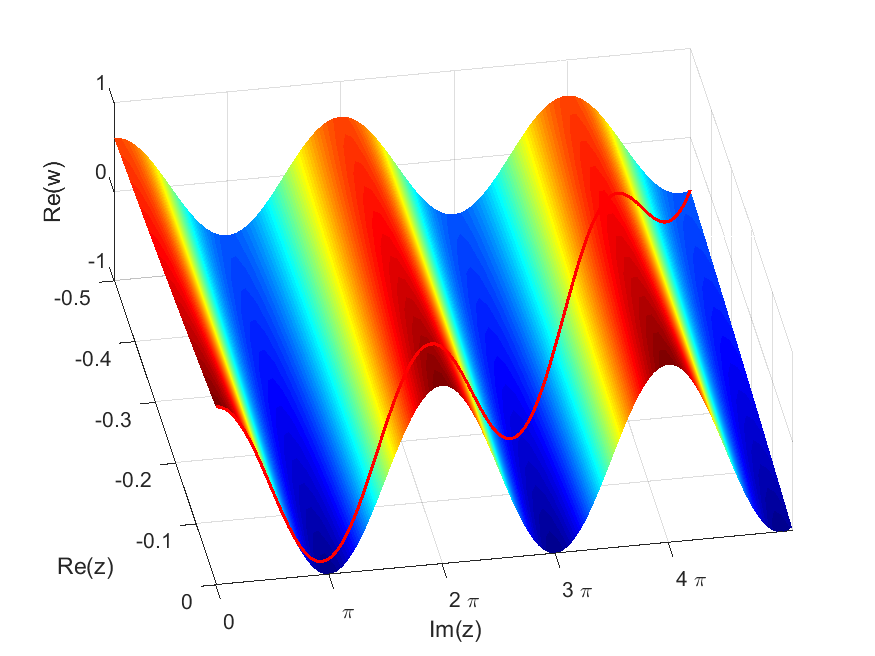
\includegraphics[width=8.5cm]{real_musg11.png}
\subcaption*{Real part with $\sigma$=1}
\end{subfigure}
\begin{subfigure}[c]{0.5\textwidth}
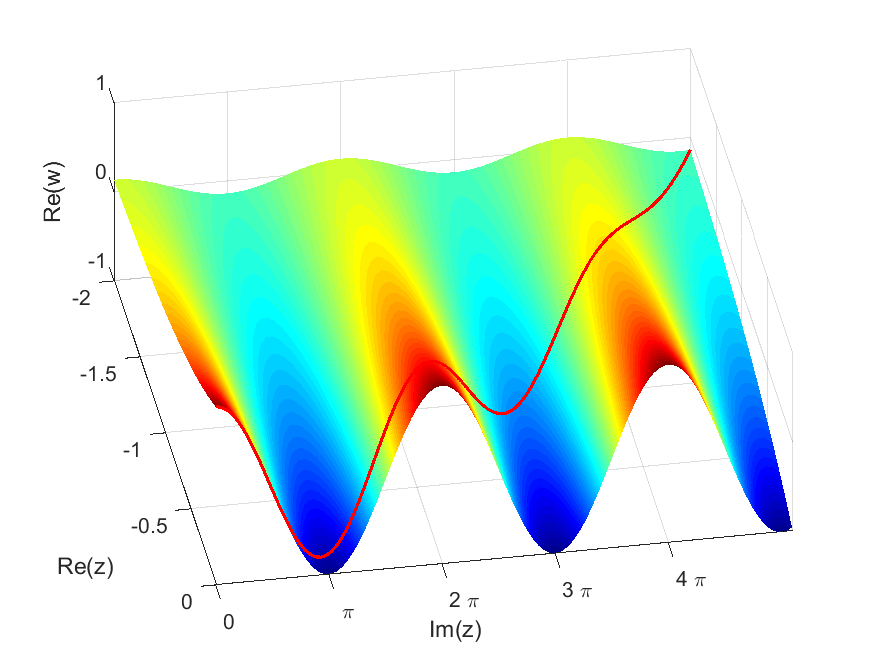
\includegraphics[width=8.5cm]{real_musg12.png}
\subcaption*{Real part with $\sigma$=2}
\end{subfigure}
\begin{subfigure}[c]{0.5\textwidth}
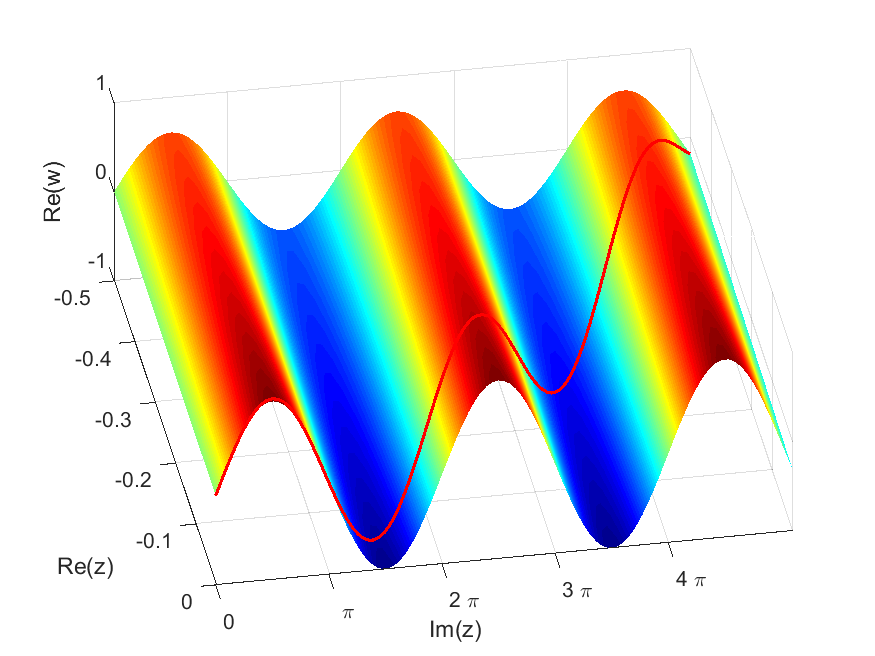
\includegraphics[width=8.5cm]{imag_musg11.png}
\subcaption*{Imaginary part with $\sigma$=1 }
\end{subfigure}
\begin{subfigure}[c]{0.5\textwidth}
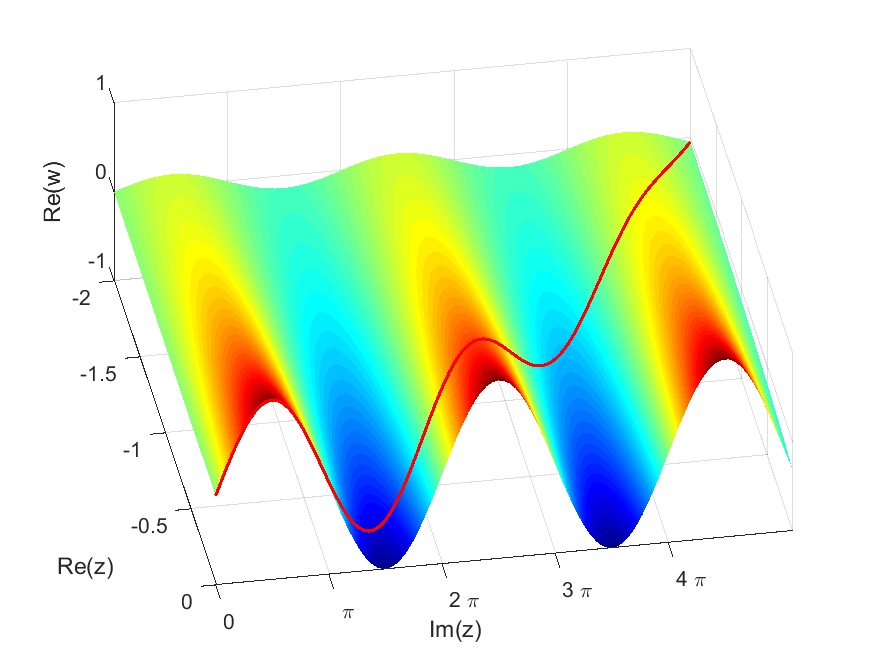
\includegraphics[width=8.5cm]{imag_musg12.png}
\subcaption*{Imaginary part with $\sigma$=2}
\end{subfigure}
\begin{subfigure}[c]{0.5\textwidth}
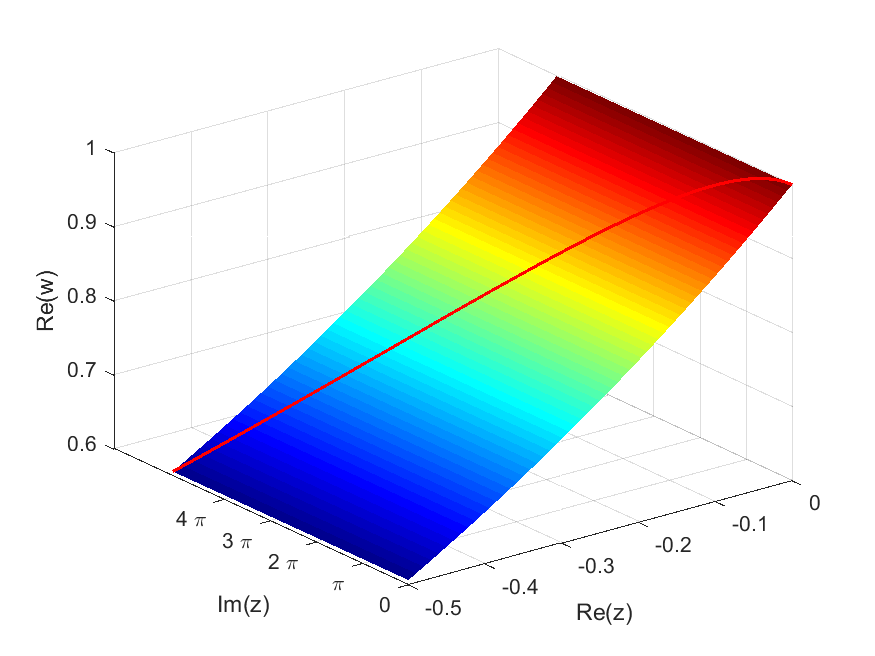
\includegraphics[width=8.5cm]{mod_musg11.png}
\subcaption*{Modulus with $\sigma$=1 }
\end{subfigure}
\begin{subfigure}[c]{0.5\textwidth}
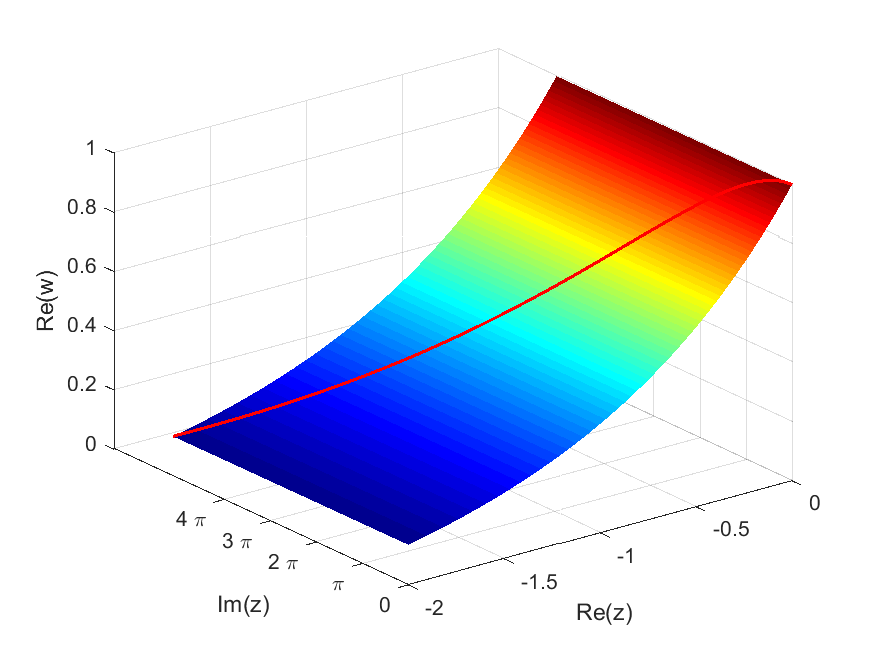
\includegraphics[width=8.5cm]{mod_musg12.png}
\subcaption*{Modulus $\sigma$=2}
\end{subfigure}
\caption{Complex Exponential function illustrations with Embedded Path for $\mu$=16}
\label{embed2}
\end{figure}
\newpage

\subsection{Technical Implementation}
In order to plot all illustrations of problem 2, one has to call the 2nd subsection of the main script \textit{$Assignment3\_MAIN.m$} where the \textit{cnorm.m} and \textit{cnorm\_embed.m} functions are called.

The script \textit{cnorm.m} basically computes the characteristic function for the given parameters by using a for-loop. These values are then plotted inside the loop.

In order to embed the functional path inside the plots of problem 1, one hast to call the function \textit{cnorm\_embed.m}. Firstly the distribution function had to be adjusted in a sense that it fits to the grid of problem 1. Again we used several for-loops to compute and plot dynamically for varying parameters $\mu$ and $\sigma$. The path of the Gaussian function was simply embedded by using the hold on command. Note that embedded illustrations above only represent a chosen $\mu$ and $\sigma$.

Note here that we made use of string arrays which is a relatively new feature of \textit{MATLAB}. With help of the \textit{stringf} commands it is possible to create strings in a loop in order create titles and save the plots dynamically. 

\section{Complex Logarithmic Function}
In this chapter we will illustrate graphically the complex logarithmic function. The complex logarithm is the inverse function of the complex exponential function, as it is the case for real numbers. Hence the logarithm of a complex number z is defined as a complex number w (Sch\"obel, 2017):
\begin{equation}
e^w=z.
\label{logder1}
\end{equation}
The principal value of the log z is defined as:
\begin{equation}
Log z = ln|z| + i Arg z
\label{arglog}
\end{equation}
Note that the complex exponential function has a non-injective feature, since for every \textit{w} with k $\in$ $\mathbb{Z}$
\begin{equation}
e^{w+2 k \pi i} = e^w
\label{elog1}
\end{equation}
From (\ref{elog1}) follows that in general all logs with respect to (\ref{logder1}) can be defined as:
\begin{equation*}
w(z)=log(z) +2k \pi i = log|z| + i (Arg z + 2k \pi i)
\end{equation*}


\subsection{Discussion of Results}
The non-injective property of the complex logarithmic function can be seen in figure \ref{logrealimag} where the left figure shows the real part and the right figure shows the imaginary part of the function. 

The real part has a specified area except of the funnel shaped area around 0 since a logarithmic function is not defined for 0. 

As you can see, the imaginary part consists of three different branches rotating  counter-clockwise since it is measured in radians\footnote{By calling the function in the code, one can see how it rotates.} and it rotates around 0 (since its not log is not defined for 0) but this this is only a restricted representation since the complex logarithm is \textit{multivalued}. In fact there are infinitely many branches which moves up or down in the plane depended on the turns of radians $2k\pi i$.  In our graph we restricted our function to k [-1 1] $\in \mathbb{Z}$. This type of illustration is also refereed as the \textit{Riemann surface} of the complex logarithmic function.

The modulus plot in \ref{logmod} shows the same behavior. The complex part is multivalued which is represented by the branches while the real part is not defined for values of 0.

The graphics in figures \ref{logcont12} and \ref{logcont34} highlight these findings. Figure \ref{logcont12} extends our surface illustrations from above with contours, whereas in figure \ref{logcont34} only these contours are considered. 

The meaning of the contours of the imaginary part of figure \ref{logcont12} get more clear if we take a look on these contours itself represented as a conformal map in figure \ref{logcont34}. The rays of the left figure illustrate the contours of only one branch (k=1), while shows how the number of rays increased with more radians k. The rays are emerging from zero and are mapped to the horizontal line of the complex plane w. The number of rays increase and rotate counter-clockwise\footnote{Again this rotation can be seen by calling the plot.}  with increasing k. Besides this, the red circle just represents the real part, which is equal to the contours of the real surface plot from above. Since this part is injective, it does not change for increasing k and remains constant.

\begin{figure}[!h]
\begin{subfigure}[c]{0.5\textwidth}
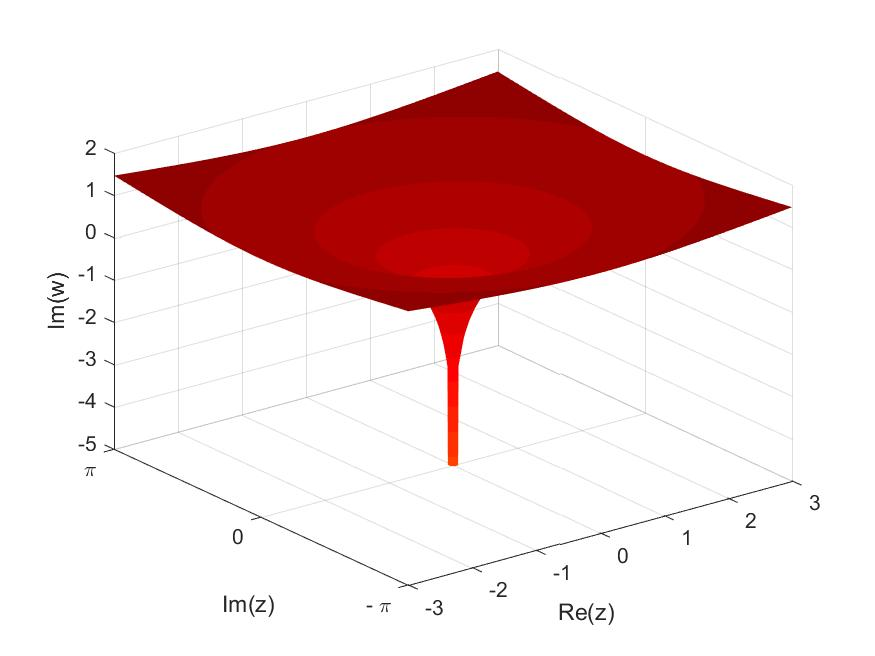
\includegraphics[width=8.5cm]{plot1_log.jpeg}
\subcaption*{Real Part}
\end{subfigure}
\begin{subfigure}[c]{0.5\textwidth}
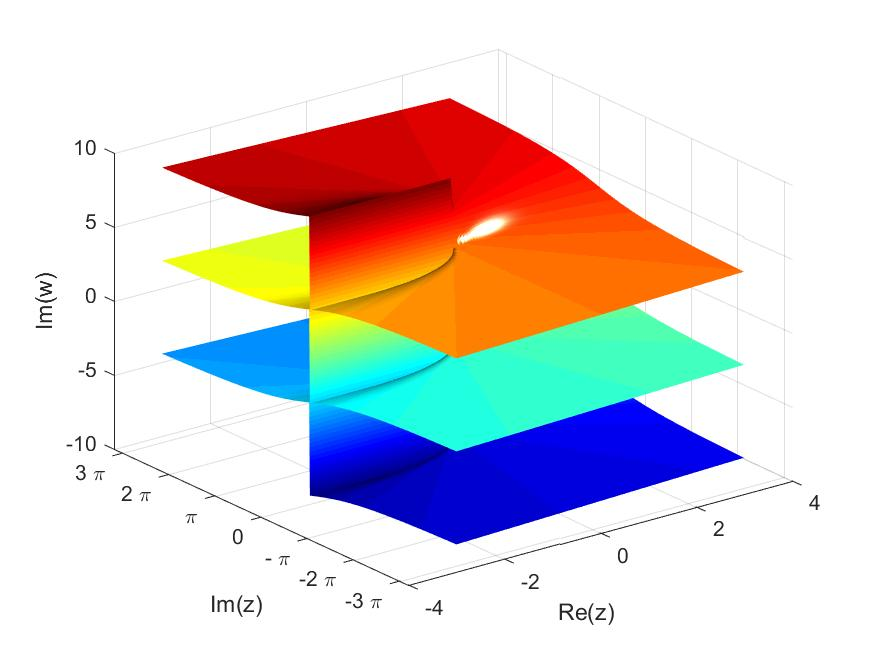
\includegraphics[width=8.5cm]{plot2_log.jpeg}
\subcaption*{Imaginary}
\end{subfigure}
\caption{Complex Logarithmic Function - Real Part and Imaginary Part}
\label{logrealimag}
\end{figure}

\begin{figure}[!h]
\begin{center}
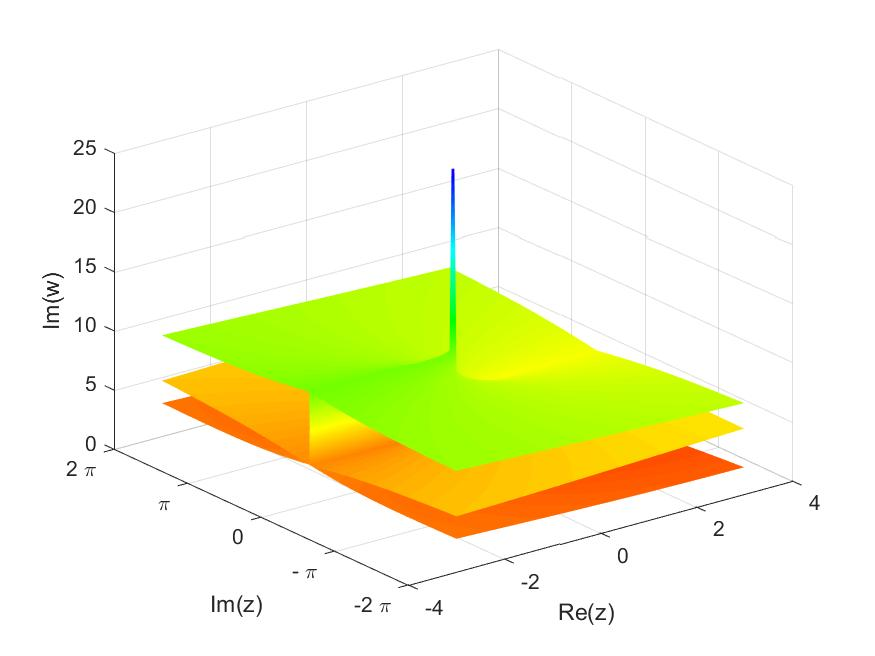
\includegraphics[width=8.5cm]{plot6_log.jpeg}
\caption{Modulus Plot of the Complex Logarithmic Function}
\label{logmod}
\end{center}
\end{figure}



\begin{figure}[!h]
\begin{subfigure}[c]{0.5\textwidth}
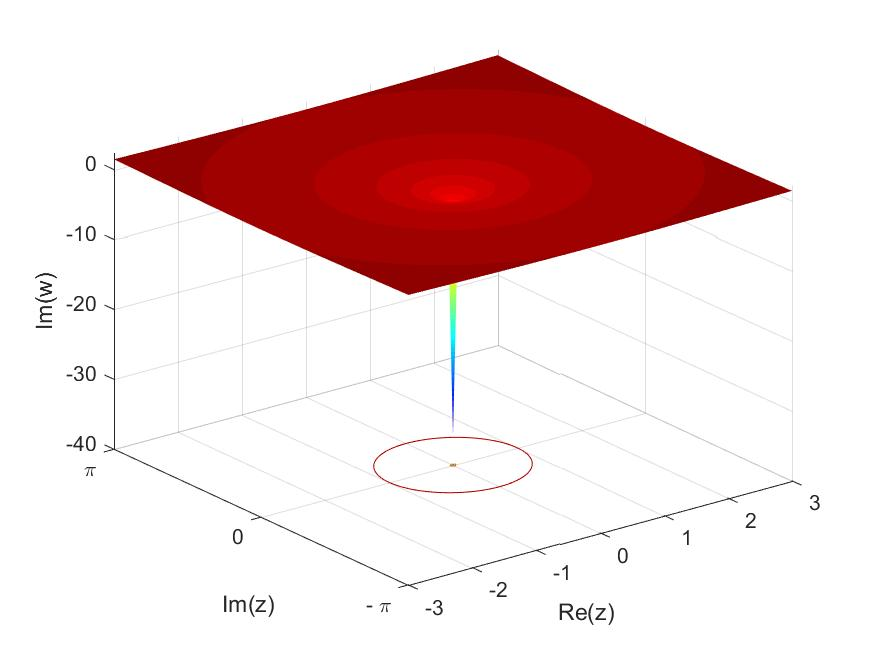
\includegraphics[width=8.5cm]{plot3_log.jpeg}
\subcaption*{Real Part}
\end{subfigure}
\begin{subfigure}[c]{0.5\textwidth}
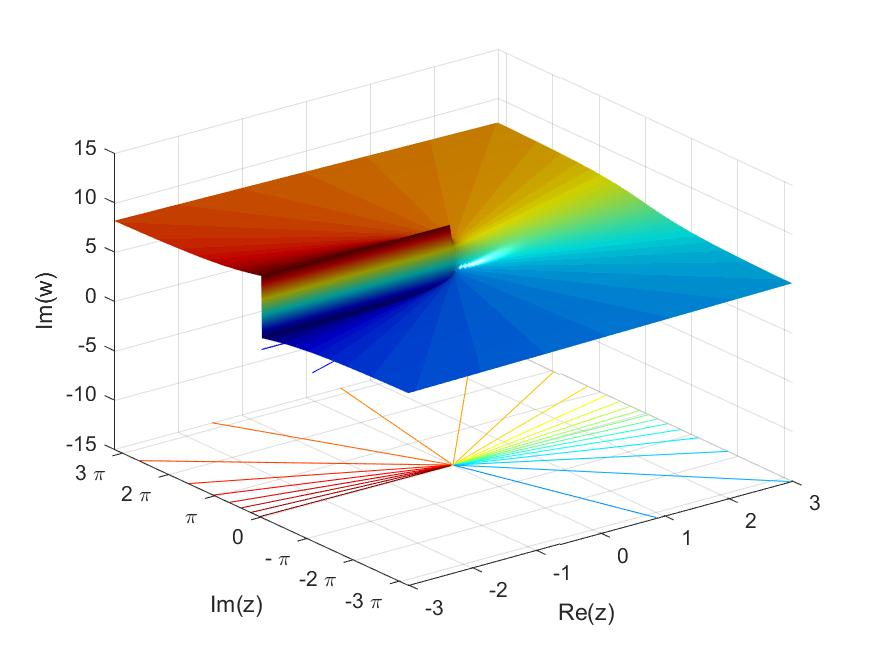
\includegraphics[width=8.5cm]{plot4_log.jpeg}
\subcaption*{Imaginary}
\end{subfigure}
\caption{Complex Logarithmic Function- Real Part and Imaginary Part with Contours}
\label{logcont12}
\end{figure}

\begin{figure}[!h]
\begin{subfigure}[c]{0.5\textwidth}
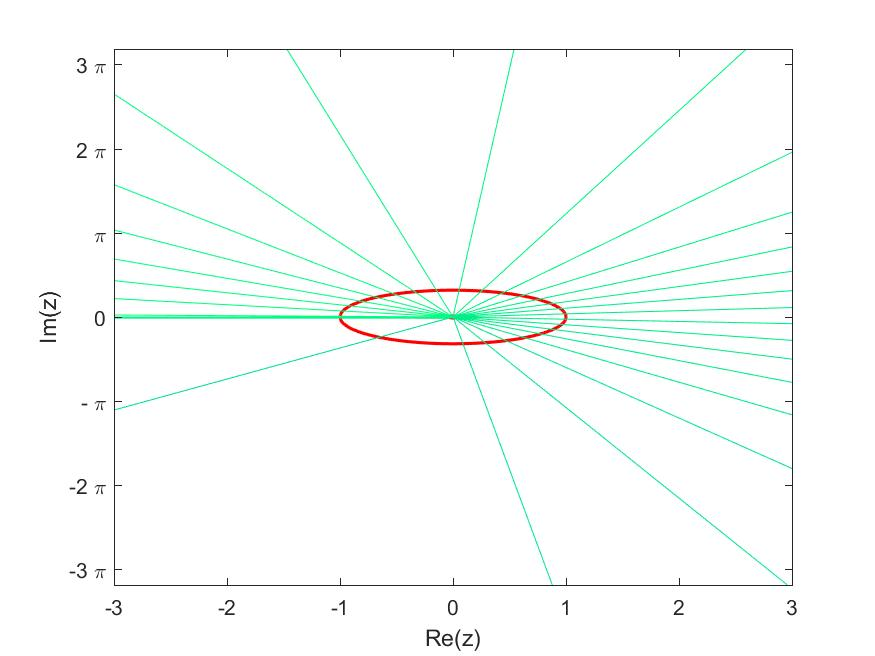
\includegraphics[width=8.5cm]{plot51_log.jpeg}
\subcaption*{k=1}
\end{subfigure}
\begin{subfigure}[c]{0.5\textwidth}
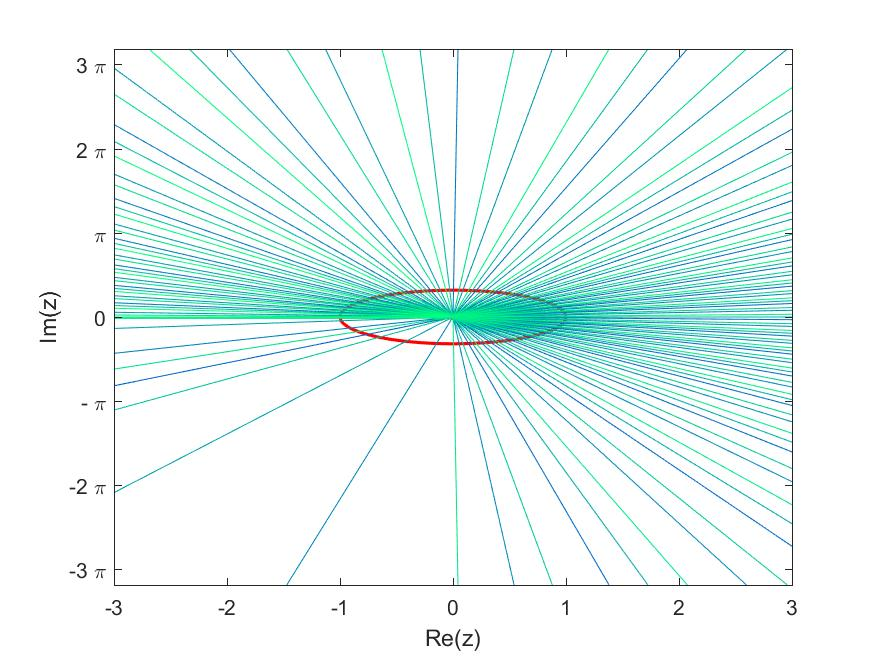
\includegraphics[width=8.5cm]{plot52_log.jpeg}
\subcaption*{k $\in \mathbb{Z}$\{[-2 2]\}}
\end{subfigure}
\caption{Conformal Map of the Complex Logarithm for different k}
\label{logcont34}
\end{figure}
\newpage


\subsection{Technical Implementation}
Again all plots can be called in the main script \textit{$Assignment3\_MAIN.m$} by calling the 3rd subsection of the script which calls the \textit{clog.m} function.

As it was the case in the exponential function we used a modified \textit{meshgrid} command to create the complex plane. To improve these illustrations we divided the grid into for quadrants and hence seperated the function into four z values. To assemble each plot for each quadrant we made use of the \textit{hold on} command.

As you can derive from the theoretical aspect, plotting of the complex logarithmic function is not trivial. The function is non-injective which means that 1:1 mapping is not possible. Hence we have to restrict the area to certain radian 'turns' by implementing a \textit{for-loop} for a chosen k. Every k increases the value of the imaginary part by one radian $2k\pi i$, as we have already derived. Again we made use of the \textit{hold on} command to assemble each step and quadrant. Hence, whenever the imaginary part of the function is plotted, the area has to be restricted by k with a for-loop. Note that it is possible to animate the construction of the imaginary parts by choosing 'Y' as an input string.
\section{Characteristic Function for Stochastic Volatility}
In this section we analyse graphically which problems the characteristic function for stochastic volatility has to face. Specifically we examine the model of Sch\"obel and Zhu (1999), in which the stochastic volatility follows a modified mean reverting Ornstein-Uhlenbeck process which additionally accounts for correlation between instantaneous volatilities and the underlying stock returns by using Fourier Inversion technique.

We focus on the characteristic function $f_2(\phi)$ which is described as:
\begin{align*}
f_2(\phi)&=\mathbb{E}^Q[exp(i \phi x(T))] \\
&= exp[i\phi(r(T-t)+x(t)) -\frac{1}{2}i\phi\rho[\sigma^{-1}v^2(t)+\sigma(T-t)]] \\
&\cdot exp[\frac{1}{2}D(t,T;\hat{s_1},\hat{s_3})v^2(t) +B(t,T;\hat{s_1},
\hat{s_2},\hat{s_3})v(t)+C(t,T;\hat{s_1},\hat{s_2},\hat{s_3})]
\end{align*} 
with the constants 
\begin{align*}
\hat{s_1} &= \frac{1}{2} \phi^2 (1-\rho^2)+ \frac{1}{2} i \phi(1-2\kappa\rho\sigma^{-1}) \\
\hat{s_2} &= i\phi\kappa\theta\rho\sigma^{-1
} \\
\hat{s_3} &= \frac{1}{2} i\phi\rho\sigma^{-1}
\end{align*}
The auxiliary functions are given by:
\begin{align*}
D(t,T)&=\frac{1}{\sigma^2}\left(\kappa - \gamma_1 \frac{sinh[\gamma_1(T-t)]+\gamma_2 cosh[\gamma_1(T-t)]}{cosh[\gamma_1(T-t)]+\gamma_2 sinh[\gamma_1(T-t)]}\right) \\ \\
B(t,T) &= \frac{1}{\sigma^2\gamma_1} \left(\frac{(\kappa\theta\gamma_1-\gamma_2 \gamma_3)+ \gamma_3(sinh[\gamma_1(T-t)] + \gamma_2 cosh[\gamma_1(T-t)])}{cosh[\gamma_1(T-t)] + \gamma_2 sinh[\gamma_1(T-t)]}-\kappa\theta\gamma_1 \right) \\ \\
C(t,T)&= -\frac{1}{2} ln(cosh[\gamma_1(T-t)] +\gamma_2 sinh[\gamma_1(T-t)])+\frac{1}{2}\kappa(T-t) \\ \\
&+ \frac{(\kappa^2\theta^2\gamma_1^{2} - \gamma_3^{2})}{2\sigma^2\gamma_1^{3}}\left(\frac{sinh[\gamma_1(T-t)]}{cosh[\gamma_1(T-t)]+\gamma_2sinh[\gamma_1(T-t)]}-\gamma_1(T-t)\right) \\ \\
&+ \frac{(\kappa\theta\gamma_1-\gamma_2\gamma_3)\gamma_3}{\sigma^2\gamma_1^{3}}\left(\frac{cosh[\gamma_1(T-t)]-1}{cosh[\gamma_1(T-t)]+\gamma_2 sinh[\gamma_1(T-t)]}\right)
\end{align*}
and the constants
\begin{align*}
\gamma_1=\sqrt{2\sigma^2s_1+\kappa^2}, \  \  \gamma_2=\frac{1}{\gamma_1}(\kappa-2\sigma^2s_3), \ \ \gamma_3=\kappa^2\theta-s_2\sigma^2
\end{align*}

\textit{
where..}

\begin{itemize}
\item S(t) = Stock price (with x(t) = lnS(t))
\item v(t) = Instantaneous volatility of stock returns
\item r = Riskless rate of return
\item $\kappa$ =  Mean reversion parameter
\item $\theta$ = Target volatility
\item $\sigma$ = Volatility of volatility
\item $\rho$ = Correlation coefficient
\item T - t = Time to maturity
\end{itemize}
\subsection{Discussion of Results}
In this problem all figures were constructed in the same manner as we did in problem 2.
Note that we only focus only on problems which the function of Sch\"obel and Zhu (1999) has to face. We will only summarize briefly the most important features of the graphical illustrations of the characteristic function before we discuss the issues. Hence only the most concise illustrations were taken into account.

As you can clearly see the plots 12 and 13 also follow a similar behavior as the plots in section 2. With increasing $\sigma$ the length of the functional paths increase.  This is not surprising because the model is an extended version of the characteristic function of the normal distribution.

What stands out immediately, are the jumps along the functional path which shows the technical issue the function faces. The frequency of the jumps increase for z and w values equally with increasing $\sigma$ and decreasing $\theta$ and increases for a correlation coefficient of $\rho$ =1. This comes from the fact that the written function does not consider the multivalued property of the complex logarithm explained in problem 3. Indeed, using only the principal value of the complex logarithm, which is the case in \textit{Matlab}, will lead to wrong integration of the characteristic function due to discontinuities in the values (Sch\"obel and Zhu, 1999).

To get the intuition of this problem recover representation (\ref{arglog}) for the complex logarithm of problem set 3:
\begin{equation*}
Log z = ln|z| + i Arg z
\end{equation*}
At some point the principal value reaches \textit{Arg}= $\pi$, or in other words, it reaches the negative real axis (we assume to come from the top). In that case, instead of increasing in $\pi$, it immediately jumps to -$\pi$ since, by definition, the principal value is only defined for (-$\pi$ $\pi$]. Same holds when we 'come from the bottom'. Hence the principal value is discontinuous at the points around the negative real axis. The issue has to be fixed manually by modifying the complex logarithmic algorithm.
\subsection{Technical Implementation}
In order to plot all illustrations of problem 4, one has to call the 4th subsection of the main script \textit{$Assignment3\_MAIN.m$} where the \textit{cvol.m function} is called.
In this function we basically adjusted the given \textit{CFSZ2.m} function, in order to compute and plot dynamically for given parameters by writing several for-loops around the logarithm. Note that in this paper we only included the most noticeable illustrations. In fact, there are 36 plots in which each plot represents a parameter combination.

Also in this function we made use of string arrays in order to plot and save dynamically.
\newpage
\begin{figure}[!h]
\begin{subfigure}[c]{0.5\textwidth}
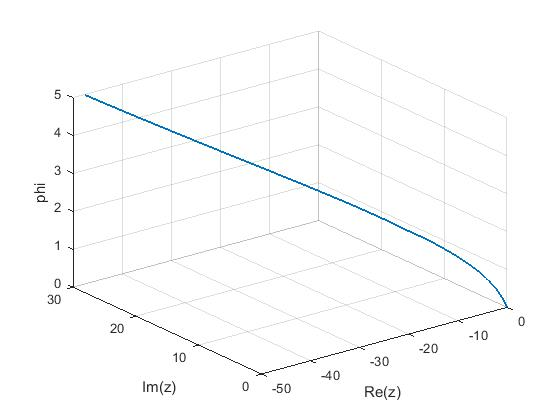
\includegraphics[width=\linewidth]{1.jpg}
\subcaption{z plane for $\rho$=0 $\sigma$=0.9 $\theta$=0.5}
\end{subfigure}
\begin{subfigure}[c]{0.5\textwidth}
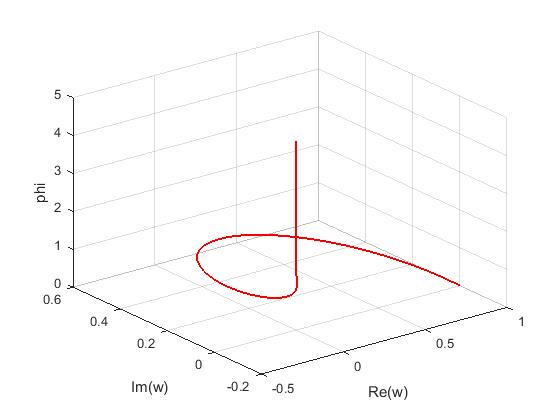
\includegraphics[width=\linewidth]{2.jpg}
\subcaption{w plane for $\rho$=0 $\sigma$=0.9 $\theta$=0.5}
\end{subfigure}
\begin{subfigure}[c]{0.5\textwidth}
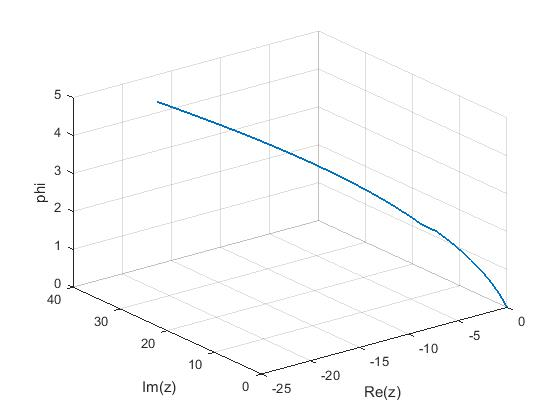
\includegraphics[width=\linewidth]{5.jpg}
\subcaption{z plane for $\rho$=0 $\sigma$=0.9 $\theta$=0}
\end{subfigure}
\begin{subfigure}[c]{0.5\textwidth}
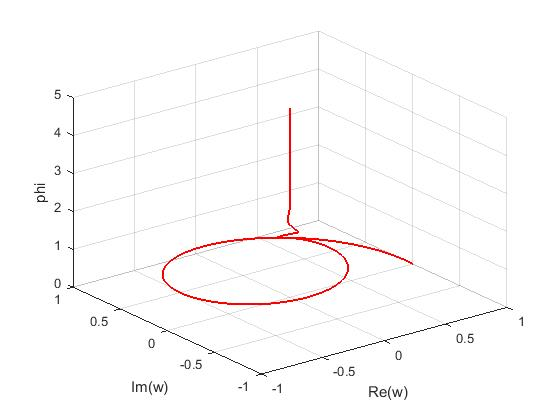
\includegraphics[width=\linewidth]{6.jpg}
\subcaption{w plane for $\rho$=0 $\sigma$=0.9 $\theta$=0}
\end{subfigure}
\begin{subfigure}[c]{0.5\textwidth}
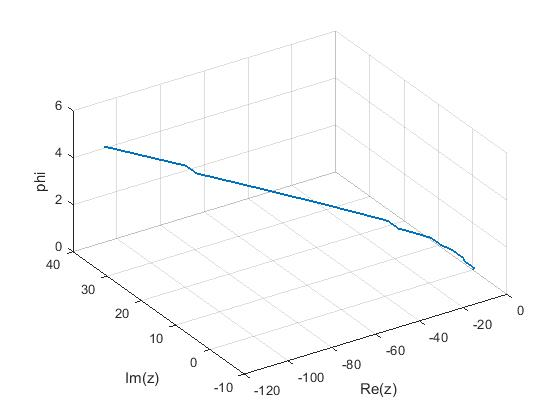
\includegraphics[width=\linewidth]{11.jpg}
\subcaption{z plane for $\rho$=0 $\sigma$=3 $\theta$=0}
\end{subfigure}
\begin{subfigure}[c]{0.5\textwidth}
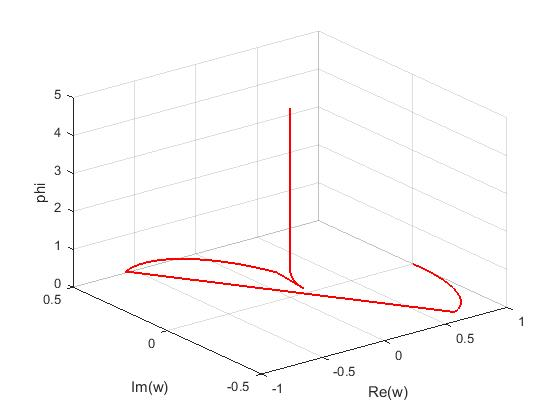
\includegraphics[width=\linewidth]{12.jpg}
\subcaption{w plane for $\rho$=0 $\sigma$=3 $\theta$=0}
\end{subfigure}
\begin{subfigure}[c]{0.5\textwidth}
\includegraphics[width=\linewidth]{17.jpg}
\subcaption{z plane for $\rho$=0 $\sigma$=9 $\theta$=0}
\end{subfigure}
\begin{subfigure}[c]{0.5\textwidth}
\includegraphics[width=\linewidth]{18.jpg}
\subcaption{w plane for $\rho$=0 $\sigma$=9 $\theta$=0}
\end{subfigure}
\caption{Illustration of the Stochastic Volatility in the z and w plane for $\rho$=0}
\label{z4}
\end{figure}

\newpage
\begin{figure}[!h]
\begin{subfigure}[c]{0.5\textwidth}
\includegraphics[width=\linewidth]{19.jpg}
\subcaption{z plane for $\rho$=0 $\sigma$=0.9 $\theta$=0.5}
\end{subfigure}
\begin{subfigure}[c]{0.5\textwidth}
\includegraphics[width=\linewidth]{20.jpg}
\subcaption{w plane for $\rho$=0 $\sigma$=0.9 $\theta$=0.5}
\end{subfigure}
\begin{subfigure}[c]{0.5\textwidth}
\includegraphics[width=\linewidth]{23.jpg}
\subcaption{z plane for $\rho$=0 $\sigma$=0.9 $\theta$=0}
\end{subfigure}
\begin{subfigure}[c]{0.5\textwidth}
\includegraphics[width=\linewidth]{24.jpg}
\subcaption{w plane for $\rho$=0 $\sigma$=0.9 $\theta$=0}
\end{subfigure}
\begin{subfigure}[c]{0.5\textwidth}
\includegraphics[width=\linewidth]{29.jpg}
\subcaption{z plane for $\rho$=0 $\sigma$=3 $\theta$=0}
\end{subfigure}
\begin{subfigure}[c]{0.5\textwidth}
\includegraphics[width=\linewidth]{30.jpg}
\subcaption{w plane for $\rho$=0 $\sigma$=3 $\theta$=0}
\end{subfigure}
\begin{subfigure}[c]{0.5\textwidth}
\includegraphics[width=\linewidth]{35.jpg}
\subcaption{z plane for $\rho$=0 $\sigma$=9 $\theta$=0}
\end{subfigure}
\begin{subfigure}[c]{0.5\textwidth}
\includegraphics[width=\linewidth]{36.jpg}
\subcaption{w plane for $\rho$=0 $\sigma$=9 $\theta$=0}
\end{subfigure}
\caption{Illustration of the Stochastic Volatility in the z and w plane for $\rho$=1}
\label{w4}
\end{figure}
\newpage
\section{References}
\

Sch\"obel, Rainer and Jianwei Zhu. \textit{Stochastic Volatility With an Ornstein-Uhlenbeck Process: An Extension.} European Finance Review 3, 1999, 23 - 46.
\\

Sch\"obel, Rainer. \textit{B473 Numerical Methods in Finance}. Lecture Script, T\"ubingen, 2017.
\end{document}